%%%%%%%%%%%%%%%%%%%%%%%%%%%%%%%%%%%%%%%%%%%%%%%%%%%%%%%%%%
% Formattazione base del documento con supporto caratteri
% accentati da tastiera win/linux e lingua italiana
%%%%%%%%%%%%%%%%%%%%%%%%%%%%%%%%%%%%%%%%%%%%%%%%%%%%%%%%%%

\documentclass[12pt,a4paper,oneside,openright]{book}

%modifico l'interlinea
\linespread{1.3}

\usepackage[utf8]{inputenc}
\usepackage[italian]{babel}

%%%%%%%%%%%%%%%%%%%%%%%%%%%%%%%%%%%%%%%%%%%%%%%%%%%%%%%%%%%%
% Pacchetto per il controllo della sintassi
% Decommentare \syntaxonly
%%%%%%%%%%%%%%%%%%%%%%%%%%%%%%%%%%%%%%%%%%%%%%%%%%%%%%%%%%

\usepackage{syntonly}
\usepackage{textcomp}
%\usepackage{dsfont}
% \syntaxonly

%%%%%%%%%%%%%%%%%%%%%%%%%%%%%%%%%%%%%%%%%%%%%%%%%%%%%%%%%%
% Inclusione pacchetto per la gestione delle figure che
% andranno copiate nella cartella figure
%
% Esempio di uso: avendo un file di nome figura1.eps questa
% si inserisce nella tesi con il comando:
%
% \begin{figure}[ht]
% \begin{center}
% \includegraphics{figura1.eps}
% \caption[nome breve]{nome lungo}
% \end{center}
% \end{figure}
%
% Il nome breve è quello che apparirà nell'indice delle
% figure ed è opzionale.
% Il nome lungo è quello che appare sotto la figura.
%%%%%%%%%%%%%%%%%%%%%%%%%%%%%%%%%%%%%%%%%%%%%%%%%%%%%%%%%%

\usepackage[final]{graphicx}
%\graphicspath{{./images/}}
\DeclareGraphicsExtensions{.png,.pdf,.jpg}

% evita il warning di pdllatex riguardo alle immagini pdf
% con versione 1.5 (al massimo 1.4 era di default..)
\pdfoptionpdfminorversion=5

% small 
\usepackage[font=small]{caption}

%\usepackage{subfigure}
%\usepackage{wrapfig}



%%%%%%%%%%%%%%%%%%%%%%%%%%%%%%%%%%%%%%%%%%%%%%%%%%%%%%%%%%
% Inclusione pacchetto per la generazione automatica
% dell'indice analitico.  Per esempio se vogliamo che la
% parola "raggruppamenti" sia indicizzata nella frase
% "I raggruppamenti sono realizzati per..." si dovrà
% scrivere "i raggruppamenti\index{raggruppamenti} ..."
%
% Compilando il file, il LaTeX produrrà un file ausiliario
% che termina con ".idx". Bisogna far processare questo
% file idx dal programma ausiliario "bibtex", che produrrâ
% a sua volta un altro file ancora. Dare infine un'ultima
% passata col LaTeX. Si può tranquillamente lasciare la
% compilazione dell'indice verso la fine della stesura del
% lavoro, quando tutto è ormai quasi definitivo.
%%%%%%%%%%%%%%%%%%%%%%%%%%%%%%%%%%%%%%%%%%%%%%%%%%%%%%%%%%

%\usepackage{makeidx}
%\usepackage{tocbibind}
%\makeindex

%%%%%%%%%%%%%%%%%%%%%%%%%%%%%%%%%%%%%%%%%%%%%%%%%%%%%%%%%%
% Numerazione delle sessioni fino alle subsub e inclusione
% nell'indice
%%%%%%%%%%%%%%%%%%%%%%%%%%%%%%%%%%%%%%%%%%%%%%%%%%%%%%%%%%

%\setcounter{secnumdepth}{4}
\setcounter{tocdepth}{4}

%%%%%%%%%%%%%%%%%%%%%%%%%%%%%%%%%%%%%%%%%%%%%%%%%%%%%%%%%%
% Inclusione pacchetto per la gestione della impostazioni
% personalizzate per la prima pagina
%%%%%%%%%%%%%%%%%%%%%%%%%%%%%%%%%%%%%%%%%%%%%%%%%%%%%%%%%%

\usepackage{unipr}
% TODO Titoli
    \titolo{Simulazione di Sistemi Fog N-Tier con Posizionamento Dinamico dei Servizi}
    \titoloIng{Simulation of N-Tier Fog Systems with Dynamic Service Placement}
    \laureando{Filippo Scaramuzza}
    \annoaccademico{2020-2021}
    \corsodilaurea{Ingegneria Informatica, Elettronica e delle Telecomunicazioni}
    \relatore[Chiar.mo Prof.]{Michele Amoretti}
    \correlatorea[Dott. Ing.]{Gabriele Penzotti}
    \dedica{Ai miei genitori.}
    %\citazione{\textit{\textquotedblleft Se ho visto più lontano, \`e perch\`e stavo sulle spalle di giganti.\textquotedblright \\ Isaac Newton}}

%%%%%%%%%%%%%%%%%%%%%%%%%%%%%%%%%%%%%%%%%%%%%%%%%%%%%%%%%%
% utilizzo il pacchetto fancyhdr per l'header e il footer
%%%%%%%%%%%%%%%%%%%%%%%%%%%%%%%%%%%%%%%%%%%%%%%%%%%%%%%%%%

\usepackage{fancyhdr}


 % Package aggiunti
  \usepackage{amssymb}				% matematica
  \usepackage{amsmath}				% matematica
  \usepackage{amsthm}				% matematica -> stile teoremi, def, proposizioni
  \usepackage{amsbsy}				% for bold math symbol
  \usepackage{cases}				% sistemi di equazioni con numerazione e sottonumerazione
  \usepackage{booktabs}				% tabelle con toprule ecc
  \usepackage{textcomp}				% per il simbolo di gradi
  \usepackage{subfig}				% per mettere pi figure in una stessa
  \usepackage[chapter]{algorithm}	% per mettere l'ambiente flottante attorno all'algoritmo (chapter \`e per la numerazione)
  \usepackage{algorithmic}			% per creare algoritmi
  \floatname{algorithm}{Algoritmo}					% opzioni dell'algoritmo: titolo in italiano
  \renewcommand{\algorithmicrequire}{\textbf{Input:}}		% require->input
  \renewcommand{\algorithmicensure}{\textbf{Output:}}	% ensure->output
  %\setlength{\parindent}{0in}			% per togliere l'indentazione all'inizio di un nuovo paragrafo

%%%%%%%%%%%%%%%%%%%%%%%%%%%%%%%%%%%%%%%%%%%%%%%%%%%%%%%%%%
% Creo un comando apposta per andare a capo con \texttt
% 
%%%%%%%%%%%%%%%%%%%%%%%%%%%%%%%%%%%%%%%%%%%%%%%%%%%%%%%%%%
  
  
\newcommand*\justify{%
  \fontdimen2\font=0.4em% interword space
  \fontdimen3\font=0.2em% interword stretch
  \fontdimen4\font=0.1em% interword shrink
  \fontdimen7\font=0.1em% extra space
  \hyphenchar\font=`\-% allowing hyphenation
}

%%%%%%%%%%%%%%%%%%%%%%%%%%%%%%%%%%%%%%%%%%%%%%%%%%%%%%%%%%
% utilizzo il pacchetto hyperref per i link nel pdf, oltretutto setto i colori dei link a nero
% nota: funziona solo con pdfLatex
%%%%%%%%%%%%%%%%%%%%%%%%%%%%%%%%%%%%%%%%%%%%%%%%%%%%%%%%%%

\usepackage[pdftex,colorlinks,plainpages=false,hyperindex,bookmarksopen,linkcolor=black,citecolor=black,urlcolor=black]{hyperref}
% pacchetto per creare i link con pdfLatex
\usepackage{hyperref}
%\hypersetup{colorlinks=true, linkcolor=black, urlcolor=black}

%%%%%%%%%%%%%%%%%%%%%%%%%%%%%%%%%%%%%%%%%%%%%%%%%%%%%%%%%%
% Definizione linguaggi nel listings
%%%%%%%%%%%%%%%%%%%%%%%%%%%%%%%%%%%%%%%%%%%%%%%%%%%%%%%%%%
\usepackage{listings}
\usepackage{xcolor}
\colorlet{punct}{red!60!black}
\definecolor{background}{HTML}{EEEEEE}
\definecolor{delim}{RGB}{20,105,176}
\colorlet{numb}{magenta!60!black}

\definecolor{maroon}{cmyk}{0, 0.87, 0.68, 0.32}
\definecolor{halfgray}{gray}{0.55}
\definecolor{ipython_frame}{RGB}{207, 207, 207}
\definecolor{ipython_bg}{RGB}{247, 247, 247}
\definecolor{ipython_red}{RGB}{186, 33, 33}
\definecolor{ipython_green}{RGB}{0, 128, 0}
\definecolor{ipython_cyan}{RGB}{64, 128, 128}
\definecolor{ipython_purple}{RGB}{170, 34, 255}

\renewcommand\lstlistingname{Listato}

\lstset{
  basicstyle=\ttfamily,
  %columns=fullflexible,
  frame=single,
  breaklines=true,
  postbreak=\mbox{\textcolor{red}{$\hookrightarrow$}\space},
}

\lstdefinelanguage{json}{
    sensitive=true,
    morecomment=[l]\#,
    morestring=[b]',
    morestring=[b]",
    morestring=[s]{'''}{'''},
    morestring=[s]{"""}{"""},
    morestring=[s]{r'}{'},
    morestring=[s]{r"}{"},
    morestring=[s]{r'''}{'''},
    morestring=[s]{r"""}{"""},
    morestring=[s]{u'}{'},
    morestring=[s]{u"}{"},
    morestring=[s]{u'''}{'''},
    morestring=[s]{u"""}{"""},
    % {replace}{replacement}{lenght of replace}
    % *{-}{-}{1} will not replace in comments and so on
    literate=
    {á}{{\'a}}1 {é}{{\'e}}1 {í}{{\'i}}1 {ó}{{\'o}}1 {ú}{{\'u}}1
    {Á}{{\'A}}1 {É}{{\'E}}1 {Í}{{\'I}}1 {Ó}{{\'O}}1 {Ú}{{\'U}}1
    {à}{{\`a}}1 {è}{{\`e}}1 {ì}{{\`i}}1 {ò}{{\`o}}1 {ù}{{\`u}}1
    {À}{{\`A}}1 {È}{{\'E}}1 {Ì}{{\`I}}1 {Ò}{{\`O}}1 {Ù}{{\`U}}1
    {ä}{{\"a}}1 {ë}{{\"e}}1 {ï}{{\"i}}1 {ö}{{\"o}}1 {ü}{{\"u}}1
    {Ä}{{\"A}}1 {Ë}{{\"E}}1 {Ï}{{\"I}}1 {Ö}{{\"O}}1 {Ü}{{\"U}}1
    {â}{{\^a}}1 {ê}{{\^e}}1 {î}{{\^i}}1 {ô}{{\^o}}1 {û}{{\^u}}1
    {Â}{{\^A}}1 {Ê}{{\^E}}1 {Î}{{\^I}}1 {Ô}{{\^O}}1 {Û}{{\^U}}1
    {œ}{{\oe}}1 {Œ}{{\OE}}1 {æ}{{\ae}}1 {Æ}{{\AE}}1 {ß}{{\ss}}1
    {ç}{{\c c}}1 {Ç}{{\c C}}1 {ø}{{\o}}1 {å}{{\r a}}1 {Å}{{\r A}}1
    {€}{{\EUR}}1 {£}{{\pounds}}1
    %
    {^}{{{\color{ipython_purple}\^{}}}}1
    {=}{{{\color{ipython_purple}=}}}1
    %
    {+}{{{\color{ipython_purple}+}}}1
    {*}{{{\color{ipython_purple}$^\ast$}}}1
    {/}{{{\color{ipython_purple}/}}}1
    %
    {+=}{{{+=}}}1
    {-=}{{{-=}}}1
    {*=}{{{$^\ast$=}}}1
    {/=}{{{/=}}}1,
    literate=
    *{-}{{{\color{ipython_purple}-}}}1
     {?}{{{\color{ipython_purple}?}}}1,
    %
    identifierstyle=\color{black}\ttfamily,
    commentstyle=\color{ipython_cyan}\ttfamily,
    stringstyle=\color{ipython_red}\ttfamily,
    keepspaces=true,
    showspaces=false,
    showstringspaces=false,
    rulecolor=\color{ipython_frame},
    frame=single,
    frameround={t}{t}{t}{t},
    framexleftmargin=6mm,
    numbers=left,
    numberstyle=\tiny\color{halfgray},
    backgroundcolor=\color{ipython_bg},
    % extendedchars=true,
    basicstyle=\scriptsize,
    keywordstyle=\color{ipython_green}\ttfamily,
    literate={\ \ }{{\ }}1
}

\lstdefinelanguage{python}{
morekeywords={access,and,break,class,continue,def,del,elif,else,except,exec,finally,for,from,global,if,import,in,is,lambda,not,or,pass,print,raise,return,try,while},
    morekeywords=[2]{abs,all,any,basestring,bin,bool,bytearray,callable,chr,classmethod,cmp,compile,complex,delattr,dict,dir,divmod,enumerate,eval,execfile,file,filter,float,format,frozenset,getattr,globals,hasattr,hash,help,hex,input,int,isinstance,issubclass,iter,len,list,locals,long,map,max,memoryview,min,next,object,oct,open,ord,pow,property,range,raw_input,reduce,reload,repr,reversed,round,set,setattr,slice,sorted,staticmethod,str,sum,super,tuple,type,unichr,unicode,vars,xrange,zip,apply,buffer,coerce,intern},
    sensitive=true,
    morecomment=[l]\#,
    morestring=[b]',
    morestring=[b]",
    morestring=[s]{'''}{'''},
    morestring=[s]{"""}{"""},
    morestring=[s]{r'}{'},
    morestring=[s]{r"}{"},
    morestring=[s]{r'''}{'''},
    morestring=[s]{r"""}{"""},
    morestring=[s]{u'}{'},
    morestring=[s]{u"}{"},
    morestring=[s]{u'''}{'''},
    morestring=[s]{u"""}{"""},
    % {replace}{replacement}{lenght of replace}
    % *{-}{-}{1} will not replace in comments and so on
    literate=
    {á}{{\'a}}1 {é}{{\'e}}1 {í}{{\'i}}1 {ó}{{\'o}}1 {ú}{{\'u}}1
    {Á}{{\'A}}1 {É}{{\'E}}1 {Í}{{\'I}}1 {Ó}{{\'O}}1 {Ú}{{\'U}}1
    {à}{{\`a}}1 {è}{{\`e}}1 {ì}{{\`i}}1 {ò}{{\`o}}1 {ù}{{\`u}}1
    {À}{{\`A}}1 {È}{{\'E}}1 {Ì}{{\`I}}1 {Ò}{{\`O}}1 {Ù}{{\`U}}1
    {ä}{{\"a}}1 {ë}{{\"e}}1 {ï}{{\"i}}1 {ö}{{\"o}}1 {ü}{{\"u}}1
    {Ä}{{\"A}}1 {Ë}{{\"E}}1 {Ï}{{\"I}}1 {Ö}{{\"O}}1 {Ü}{{\"U}}1
    {â}{{\^a}}1 {ê}{{\^e}}1 {î}{{\^i}}1 {ô}{{\^o}}1 {û}{{\^u}}1
    {Â}{{\^A}}1 {Ê}{{\^E}}1 {Î}{{\^I}}1 {Ô}{{\^O}}1 {Û}{{\^U}}1
    {œ}{{\oe}}1 {Œ}{{\OE}}1 {æ}{{\ae}}1 {Æ}{{\AE}}1 {ß}{{\ss}}1
    {ç}{{\c c}}1 {Ç}{{\c C}}1 {ø}{{\o}}1 {å}{{\r a}}1 {Å}{{\r A}}1
    {€}{{\EUR}}1 {£}{{\pounds}}1
    %
    {^}{{{\color{ipython_purple}\^{}}}}1
    {=}{{{\color{ipython_purple}=}}}1
    %
    {+}{{{\color{ipython_purple}+}}}1
    {*}{{{\color{ipython_purple}$^\ast$}}}1
    {/}{{{\color{ipython_purple}/}}}1
    %
    {+=}{{{+=}}}1
    {-=}{{{-=}}}1
    {*=}{{{$^\ast$=}}}1
    {/=}{{{/=}}}1,
    literate=
    *{-}{{{\color{ipython_purple}-}}}1
     {?}{{{\color{ipython_purple}?}}}1,
    %
    identifierstyle=\color{black}\ttfamily,
    commentstyle=\color{ipython_cyan}\ttfamily,
    stringstyle=\color{ipython_red}\ttfamily,
    keepspaces=true,
    showspaces=false,
    showstringspaces=false,
    rulecolor=\color{ipython_frame},
    frame=single,
    frameround={t}{t}{t}{t},
    framexleftmargin=6mm,
    numbers=left,
    numberstyle=\tiny\color{halfgray},
    backgroundcolor=\color{ipython_bg},
    % extendedchars=true,
    basicstyle=\scriptsize,
    keywordstyle=\color{ipython_green}\ttfamily,
    literate={\ \ }{{\ }}1
}

%%%%%%%%%%%%%%%%%%%%%%%%%%%%%%%%%%%%%%%%%%%%%%%%%%%%%%%%%%
% Comandi aggiuntivi
%%%%%%%%%%%%%%%%%%%%%%%%%%%%%%%%%%%%%%%%%%%%%%%%%%%%%%%%%%
%\newcommand{\EQ}[1]{Eq.~(\ref{#1})}
%\newcommand{\BEGMATRIX}[1]{\left[\begin{array}{#1}}
%\newcommand{\ENDMATRIX}{\end{array}\right]}
%\def\argmin{\mathop{\rm argmin}}

%%%%%%%%%%%%%%%%%%%%%%%%%%%%%%%%%%%%%%%%%%%%%%%%%%%%%%%%%%
% Corpo della tesi
%%%%%%%%%%%%%%%%%%%%%%%%%%%%%%%%%%%%%%%%%%%%%%%%%%%%%%%%%%

\begin{document}

% PAGE HEADERS permette di creare gli header delle pagine con il numero, il capitolo e la riga sotto
\pagestyle{fancy}
\headheight 15pt
\renewcommand{\chaptermark}[1]{\markboth{{\chaptername}\ \thechapter.\hspace{1em}#1}{}}
\renewcommand{\footrulewidth}{0pt}
% definisce l'header e il footer
\lhead[\fancyplain{}{}]{\fancyplain{}{\leftmark}} \chead{}
\rhead{\thepage} \lfoot{} \cfoot{} \rfoot{}

% definizione dei teoremi, proposizioni, definizioni ecc usato con il package amsthm
	\newtheorem{definizione}{Definizione}[chapter] 		% il chapter si usa per la sotto numerazione nei capitoli
	\newtheorem{proposizione}{Proposizione}[chapter]
	\newtheorem{problema}{Problema}[chapter]
	\newtheorem{proprieta}{Propriet\`a}[chapter]


%%%%%%%%%%%%%%%%%%%%%%%%%%%%%%%%%%%%%%%%%%%%%%%%%%%%%%%%%%
% Inizio della parte introduttiva
%%%%%%%%%%%%%%%%%%%%%%%%%%%%%%%%%%%%%%%%%%%%%%%%%%%%%%%%%%
\maketitle 


\frontmatter
\pagenumbering{alph}



\chapter*{Ringraziamenti}

Ringrazio innanzitutto il prof. Amoretti per avermi dato la possibilità di intraprendere il percorso di Internato di Laboratorio da cui è nato questo lavoro di Tesi. Allo stesso modo ringrazio immensamente Gabriele Penzotti per il suo aiuto fondamentale, sia durante i mesi di Internato di Laboratorio, sia durante la fase di stesura di queste pagine.

Voglio ringraziare la mia famiglia, che mi ha dato la possibilità di studiare e di aprire la mia mente come mai avrei pensato. Il loro supporto, in ogni momento di questi 3 impegnativi anni, è stato fondamentale. Vorrei anche scusarmi per tutti i momenti di totale delirio nei momenti antecedenti agli esami con coloro che mi hanno dovuto sopportare e che, purtroppo o per fortuna dovranno continuare a farlo.

Infine voglio ringraziare gli amici da una vita, Letizia e Nicolò, i compagni di classe prima, di Università poi, Luca e Davide, che hanno condiviso con me giornate di studio matto e di grandi gioie. 

Ringrazio quindi tutte le persone, vicine e non, che mi hanno permesso, anche involontariamente, di arrivare a questo punto della mia carriera universitaria e della mia vita. Grazie di tutto.

\pagenumbering{roman}
\tableofcontents
%\listoffigures


%\lstlistoflistings


%%%%%%%%%%%%%%%%%%%%%%%%%%%%%%%%%%%%%%%%%%%%%%%%%%%%%%%%%%
% Inizio della parte centrale
%%%%%%%%%%%%%%%%%%%%%%%%%%%%%%%%%%%%%%%%%%%%%%%%%%%%%%%%%%
% \pagenumbering{arabic}
\mainmatter

\chapter*{Introduzione} % \chapter* -> the introduction isn't the Chapter 1, it's not a numbered chapter
\addcontentsline{toc}{chapter}{Introduzione} %this line enable the introduction to be listed in the Table Of Contents even if it's not a numbered chapter (see above)
\markboth{}{}

Nell'era dei Big Data il tempo richiesto per accedere ad alcune applicazioni \textit{Cloud-based}, che concentrano l'intera elaborazione dei dati nei \textit{data center}, potrebbe essere troppo elevato. Inoltre, l'ormai noto incremento dei dispositivi connessi in ambito Internet of Things, ed il conseguente rapido aumento dei dati generati nell'edge della rete richiedono l'implementazione del cosiddetto \textit{Cloud-to-Thing Continuum}. In questo ambito sono state avanzate numerose proposte, ad esempio il \textit{Fog Computing}, un paradigma a livello di sistema che distribuisce le funzioni di elaborazione, archiviazione, controllo e comunicazione dall'edge al Cloud. \cite{OpenFogReferenceArchitecture}. I possibili ambiti di applicazione del \textit{Fog Computing} sono innumerevoli: dagli \textit{Smart Vehicles} al \textit{Traffic Control}, alle \textit{Smart Cities} e agli \textit{Smart Buildings}.

Questo lavoro di Tesi nasce da un periodo di Internato di Laboratorio presso il Dipartimento di Ingegneria e Architettura dell'Università di Parma, il cui obiettivo è stato quello di realizzare simulazioni di sistemi Fog, con lo scopo di poter analizzare questo paradigma in un'architettura \textit{N-Tier}, implementando anche uno specifico algoritmo di placement dei servizi.

L'architettura di riferimento ha una struttura composta da 3 macro-entità: il Cloud, il livello Fog e gli end-node/dispositivi IoT. Il livello Fog, inoltre, è ulteriormente scomposto in sotto-livelli (tier) che più sono distanti dai dispositivi, più aumentano le loro capacità computazionali.

Il software realizzato si basa su \textit{YAFS} (\textit{Yet Another Fog Simulator}), un simulatore ad eventi discreti sviluppato in Python ed a sua volta basato su \textit{SimPy}, ovvero un framework DES (\textit{Discrete Event Simulator}) basato sui processi, anch'esso sviluppato in Python. Nel \textit{Capitolo 1} vengono introdotti i principali concetti fondanti del \textit{Cloud Computing}, del \textit{Fog Computing} e degli altri principali paradigmi in quest'ambito di ricerca. Vengono poi citate possibili applicazioni del \textit{Fog Computing} e viene fatta una breve introduzione a YAFS. Nel \textit{Capitolo 2} vengono affrontati i dettagli implementativi del simulatore YAFS, la sua struttura e la modellazione delle simulazioni. Successivamente vengono approfondite le caratteristiche degli scenari simulati in questo lavoro di Tesi. Nel \textit{Capitolo 3} vengono trattati i principali aspetti del sistema di simulazione realizzato. Vengono poi discusse le modalità di utilizzo e le analisi che si possono eseguire. Nel \textit{Capitolo 4}, vengono presentati i principali risultati ottenuti dalle simulazioni eseguite. Vengono in particolare valutati l'algoritmo di placement utilizzato al variare di specifici parametri di configurazione del sistema ed il soddisfacimento delle richieste con e senza failure control. In conclusione, vengono discussi il lavoro svolto e i possibili sviluppi futuri.




 \clearpage
         \chapter{Stato dell'Arte}

In questo capitolo si introdurranno i principali concetti utili ad una comprensione generale degli aspetti fondanti del \textit{Cloud Computing}, \textit{Fog Computing} e degli altri principali paradigmi in quest'ambito di ricerca. Verranno poi citate alcune possibili applicazioni del \textit{Fog Computing} e verrà fatta una breve introduzione a \textit{YAFS}, il simulatore utilizzato per analizzare generalizzazioni dei suddetti scenari.

\section{Cloud Computing nell'Era dei Big Data}

Il NIST (\textit{National Institute of Standards and Technology}) definisce il \textit{Cloud Computing} come un modello che promuove l'accesso globale alle risorse informatiche condivise, tipicamente \textit{on-demand} \cite{NISTCloudComputing}. L'infrastruttura di questo paradigma, nella sua versione più semplice, è relegata principalmente in \textit{data center}, ovvero dei raggruppamenti di risorse virtualizzate altamente accessibili che possono essere riconfigurate dinamicamente per garantire la scalabilità dei servizi. Questi fungono da nodi centrali e garantiscono agli utenti un'infrastruttura, una piattaforma oppure un servizio software utile per le loro applicazioni e i propri scopi (IaaS, Paas, SaaS).

Nonostante il \textit{Cloud Computing} abbia indubbiamente un ruolo chiave nel rendere accessibile una potenza di calcolo altrimenti troppo difficile da poter essere realizzata in proprio, nella moderna era dei Big Data il tempo richiesto per accedere ad alcune applicazioni \textit{Cloud-based}, che concentrano l'intera elaborazione dei dati nei suddetti \textit{data center}, potrebbe essere troppo elevato e rendere questo paradigma impraticabile per applicazioni \textit{real-time} o, in generale, ovunque la latenza debba essere ridotta al minimo. Inoltre l'ormai noto incremento dei dispositivi connessi in ambito IoT (\textit{Internet of Things}) ed il relativo rapido aumento dei dati generati nell'\textit{edge}\footnote{Con \textit{edge} si intende la zona perimetrale della rete, in cui risiedono gli end-node. L'edge è caratterizzato da un punto di demarcazione (ad esempio un \textit{gateway}) che lo separa dal \textit{network core}, ovvero la parte centrale gestita dagli Internet Service Provider.} della rete richiedono che le risorse di calcolo siano geograficamente situate il più vicino possibile ai dispositivi stessi, così da diminuire al massimo la latenza, aumentando di conseguenza il \textit{throughput} della rete.

Per affrontare queste problematiche è quindi necessario garantire il cosiddetto \textit{Cloud-to-Thing Continuum}, ovvero la possibilità di rendere disponibili potenza computazionale, di storage e di networking ovunque nella rete, dal Cloud agli end-nodes. In questo ambito sono state avanzate numerose proposte, ad esempio il \textit{Fog Computing}, sia in ambito industriale che accademico \cite{OpenFogReferenceArchitecture, FogComputingInIoT}.

\section[Fog Computing ed Altri Paradigmi nel Cloud-to-Thing Continuum]{Fog Computing ed altri paradigmi nel \\Cloud-to-Thing Continuum}

Con \textit{Fog Computing} si intende un'architettura a livello di sistema che distribuisce le funzioni di elaborazione, archiviazione, controllo e rete più vicine agli utenti lungo un \textit{Cloud-to-Thing Continuum} \cite{OpenFogReferenceArchitecture}.

Il \textit{Fog Computing} dunque è innanzitutto caratterizzato da un approccio distribuito. Ciò deriva dal bisogno di superare i limiti dell'approccio centralizzato del Cloud Computing, come latenza, privacy e sovraccarico dei dati. In secondo luogo, i nodi Fog possono essere posizionati ovunque nella rete tra gli end-node e il Cloud \cite{CloudComputingBigDataIssues}. Questa flessibilità che contraddistingue il Fog Computing sottolinea la visione di questo paradigma non come una sostituzione, bensì come un'estensione del Cloud Computing, con lo scopo di colmare il divario tra quest'ultimo e i dispositivi IoT, garantendo quindi il continuum \textit{Cloud-to-Thing}.

Ad esempio, in un'applicazione che si occupa di analisi di Big Data prodotti da migliaia di dispositivi IoT, lo strato di Fog che si pone ad un livello "più basso", ovvero più vicino ai dispositivi  rispetto al Cloud, potrebbe svolgere una funzione di filtraggio, pre-elaborazione e aggregazione del flusso dati, rendendo eventualmente disponibili alcuni risultati ai livelli inferiori e alleggerendo il carico nel Cloud, a cui rimarrebbero i task più complessi ma su una mole di dati molto ridotta e pre-elaborata.

\begin{figure}[!ht]
  \includegraphics[width=12cm]{images/FogCloudToThingContinuum}
  \centering
  \caption[Architettura OpenFog N-Tier]{Architettura OpenFog N-Tier. \cite{OpenFogReferenceArchitecture}}
  \label{fig:ntier_architecture}
\end{figure}

Negli anni sono state proposte alcune architetture di particolare rilievo per scenari di Fog Computing. Molte ricerche fanno riferimento ad un'architettura a 3 livelli, composta da Cloud, Fog e IoT \cite{ThreeLevelArchitecture}. Per questo lavoro di Tesi l'architettura di riferimento è quella fornita dall'\textit{OpenFog Consortium}. Quest'ultimo è stato fondato da ARM, Cisco, Dell, Intel, Microsoft e dall'Università di Princeton, nel 2015. Ad oggi OpenFog e i suoi membri fanno parte dell'\textit{IIC} (\textit{Industrial Internet Consortium}). 

L'architettura di riferimento è detta \textit{N-Tier Architecture}, il cui schema è mostrato in Figura \ref{fig:ntier_architecture}. Questa mantiene comunque una struttura composta da tre macro-entità: il Cloud, il livello Fog e gli end-node/dispositivi IoT. Il livello Fog, però, è ulteriormente scomposto in sotto-livelli (\textit{tier}) che più si allontanano dai dispositivi, più aumentano le loro capacità computazionali. Il numero di livelli Fog da adottare dipende dai requisiti dello scenario secondo diversi parametri, ad esempio il numero di dispositivi IoT, il carico di lavoro, le capacità dei nodi ad ogni livello, i requisiti di latenza minima e così via. Inoltre i nodi Fog in ogni \textit{tier} possono essere collegati tra loro formando una maglia capace di fornire caratteristiche aggiuntive, come resilienza, tolleranza ai guasti, bilanciamento del carico e così via. Questo significa che i nodi sono in grado di comunicare sia orizzontalmente che verticalmente all'interno dell'architettura Fog.

I vantaggi fondamentali dell'architettura di riferimento definita dall'OpenFog Consortium sono riassunti con il termine \textit{SCALE} \cite{OpenFogReferenceArchitecture}, ovvero:

\begin{itemize}
	\item \textbf{Security}. Sicurezza aggiuntiva per garantire transazioni sicure e affidabili. Dal \textit{Security Pillar} dell'architettura di riferimento, si evince la necessità di uno o più "nodi fidati" (\textit{Root of Trust}) quando si trattano dati sensibili.
	\item \textbf{Cognition}. L'infrastruttura Fog è consapevole dei requisiti e degli obiettivi delle applicazioni, quindi distribuisce le capacità di elaborazione, comunicazione, controllo e archiviazione lungo il continuum Cloud-to-Things, creando applicazioni che soddisfano meglio le esigenze specifiche dello scenario.
	\item \textbf{Agility}. Lo sviluppo di un nuovo servizio è solitamente lento e costoso, a causa dei costi e dei tempi necessari ai grandi fornitori per avviare o adottare l'innovazione. Il Fog Computing, invece, offre innovazione rapida e scalabilità conveniente, in cui individui e piccoli team possono utilizzare strumenti di sviluppo aperti (ad esempio API e SDK, secondo il pilastro \textit{Openness} definito da OpenFog \cite{OpenFogReferenceArchitecture}) e la proliferazione di dispositivi IoT per offrire nuovi servizi.
	\item \textbf{Latency}. L'architettura Fog supporta l'elaborazione e l'archiviazione dei dati vicino all'utente, con conseguente bassa latenza. Pertanto, il Fog computing soddisfa perfettamente la richiesta di elaborazione in tempo reale, in particolare quindi per le applicazioni \textit{real-time}.
	\item \textbf{Efficiency}. Riconoscimento e condivisione delle risorse inutilizzate dei dispositivi finali che partecipano al networking.
\end{itemize}

\subsection{Possibili Applicazioni del Fog Computing}

\subsubsection{Smart Vehicles e Traffic Control}

I veicoli smart (\textit{Smart Vehicles}) sono in grado di produrre giornalmente svariati terabyte di dati grazie alla combinazione di sensori \textit{LIDAR}\footnote{LIDAR (\textit{Light Detection and Ranging}) è un metodo per determinare la presenza di oggetti, la loro forma e la loro distanza dall'osservatore utilizzando un laser e misurando il tempo necessario alla luce riflessa per tornare al trasmettitore laser.}, dei sensori GPS, delle videocamere intelligenti a bordo dei veicoli per il riconoscimento delle immagini e così via. Oltre ai dati prodotti dagli \textit{Smart Vehicles} ci sono quelli generati dai sistemi di controllo intelligenti, ovvero l'infrastruttura del \textit{Traffic Control} (semafori intelligenti, sensori di rilevamento del traffico e delle congestioni, videocamere, ecc.). È evidente come un modello \textit{Cloud-only} non sia adatto, vista l'enorme mole di dati, a garantire un throughput sufficientemente elevato. In quest'ambito è inoltre estremamente importante avere latenze ridotte al minimo, vista la natura \textit{real-time} di molti vincoli decisionali \cite{RealTimeDecisionMakingSmartVehicles}. Un'architettura Fog potrebbe soddisfare le particolari esigenze di questo scenario. In quest'ultimo i nodi Fog a bordo degli \textit{Smart Vehicles} possono offrire i normali servizi di \textit{infotainment}, ADAS\footnote{ADAS (\textit{Advanced Driver Assistance Systems}) è un insieme di tecnologie che assistono il guidatore nelle operazioni di guida e parcheggio in modo sicuro.}, guida autonoma, sistemi anticollisione, navigazione, e così via, comunicando per mezzo di diverse tecnologie, come DSRC (\textit{Dedicated Short Range Communications}) o le reti cellulari (3G, LTE, 5G, ecc.).

\begin{figure}[!ht]
  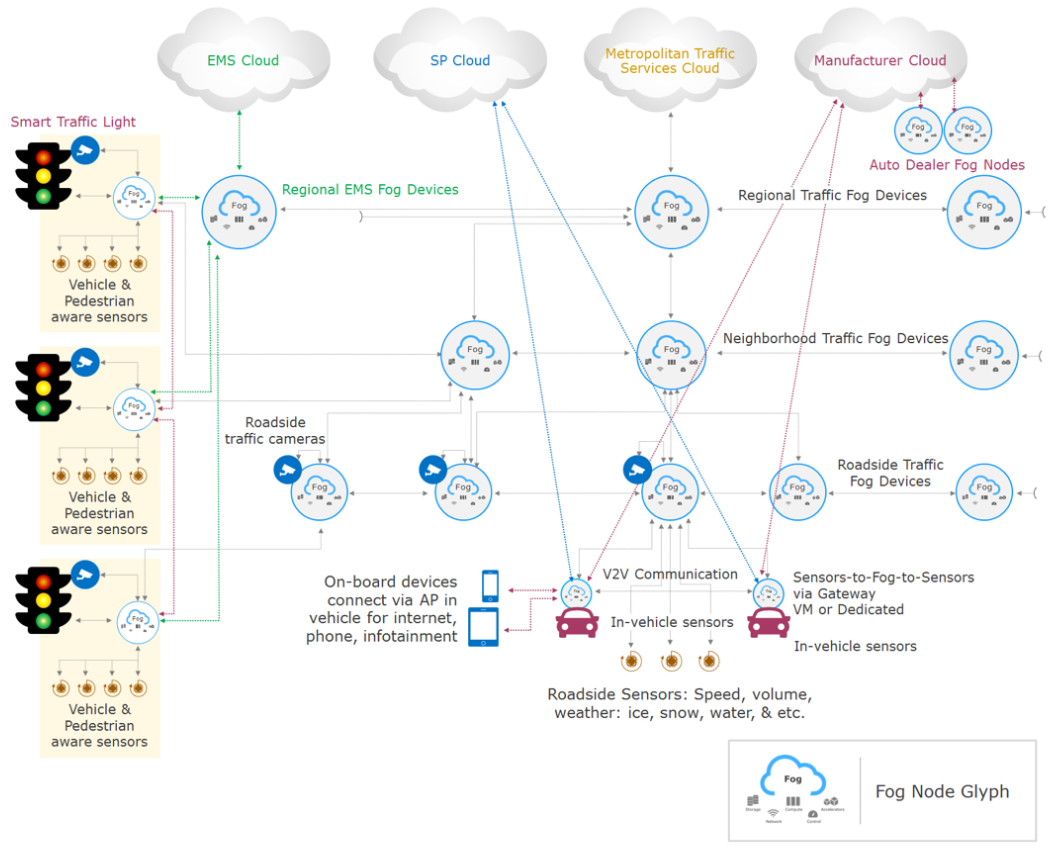
\includegraphics[width=14cm]{images/smartcars_trafficcontrol}
  \centering
  \caption[Architettura di uno scenario Fog in ambito Smart Vehicles e Traffic Control]{Architettura di uno scenario Fog in ambito Smart Vehicles e Traffic Control. \cite{OpenFogReferenceArchitecture}}
  \label{fig:smartcars_trafficcontrol}
\end{figure}

L'architettura di riferimento, mostrata in Figura \ref{fig:smartcars_trafficcontrol}, è strutturalmente gerarchica, con 3 livelli di nodi Fog. Il primo livello (\textit{Roadside Fog Nodes}) si occupa di raccogliere i dati dai vari sensori e telecamere. I nodi Fog in questo livello eseguono alcune veloci analisi, utili ad esempio a comunicare ai veicoli in transito particolari condizioni del traffico o della strada. I dati aggregati dal primo livello sono inviati al secondo e/o al terzo livello (non c'è necessariamente una gerarchia nelle comunicazioni, questo per definizione dell'architettura Fog e della sua flessibilità), ovvero i \textit{Neighborhood Fog Nodes} e i \textit{Regional Fog Nodes}. In genere, ogni livello Fog nella gerarchia fornisce ulteriori capacità di elaborazione, storage e rete. Ad esempio, livelli gerarchicamente più alti garantiscono un trattamento aggiuntivo per fornire analisi dei dati o capacità di archiviazione di grandi dimensioni, utili ad esempio per analisi sul lungo periodo o per inviare dati ad altre zone della rete stradale per particolari task.

\subsubsection{Smart Cities e Smart Buildings}

Un altro interessante impiego del Fog Computing è nell'ambito delle \textit{Smart Cities} e degli \textit{Smart Buildings}. Infatti sebbene  la maggior parte delle città moderne disponga di una o più reti cellulari che forniscono una copertura dell'intera città, queste reti hanno spesso limiti di capacità e larghezza di banda che soddisfano appena le esigenze degli attuali abbonati. Ciò lascia poca larghezza di banda per i servizi più avanzati previsti in una città intelligente nell'era dei Big Data, come \textit{Smart Parking}, \textit{Traffic Control}, ospedali intelligenti, controllo sul consumo elettrico e così via.  

\begin{figure}[!ht]
  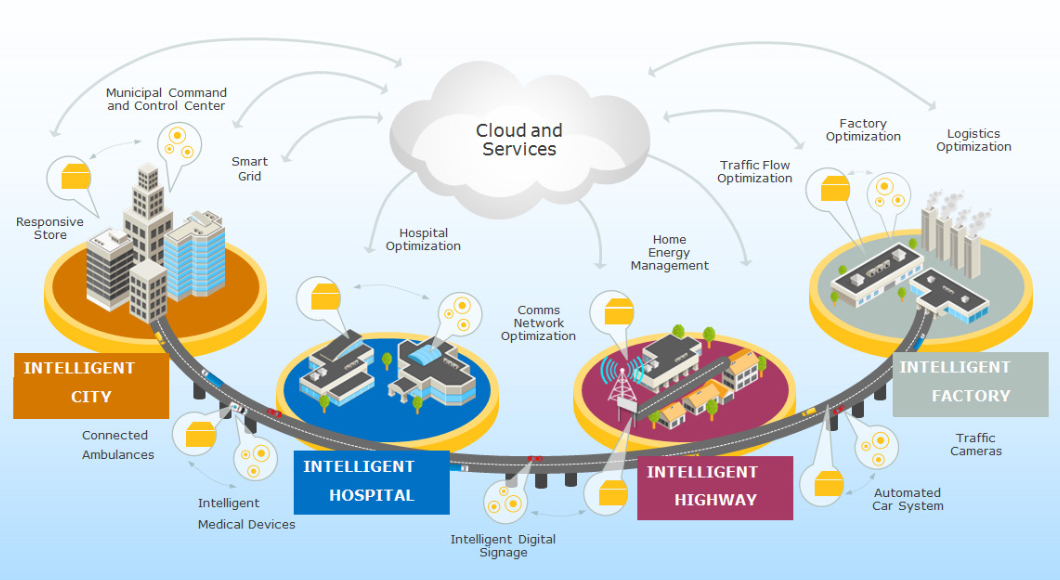
\includegraphics[width=14cm]{images/smartcities_smartbuildings}
  \centering
  \caption[Opportunità per una Smart City]{Opportunità per una \textit{Smart City}. \cite{OpenFogReferenceArchitecture}}
  \label{fig:smartcities_smartbuildings}
\end{figure}


Questo caso d'uso è già realtà, ad esempio, nella città di Barcellona, dove i risultati hanno dimostrato che il Fog Computing è la possibile chiave di volta per l'implementazione di servizi molto avanzati e complessi, in città che producono decine di milioni di Gigabyte di dati giornalmente \cite{FogBarcellona}. 

\subsection{Altri Paradigmi}

Per analizzare i vari altri paradigmi che possono essere considerati un'estensione, più che un'alternativa al Fog Computing, è utile introdurre il concetto di \textit{Edge Computing}. Quest'ultimo è un un paradigma nato dall'esigenza di spostare la capacità di calcolo verso l'edge della rete. In \cite{EdgeComputing} viene definito l'Edge Computing come \textit{"tecnologie abilitanti che consentono di effettuare calcoli ai margini della rete sui dati, a valle per conto di servizi Cloud e a monte per conto di servizi IoT"}. L'idea è quella di estendere le capacità dal Cloud all'edge della rete, con l'obiettivo di portare la potenza di calcolo il più vicino possibile ai generatori dei dati, ovvero ai dispositivi IoT. Nonostante sia il Fog Computing che l'Edge Computing muovano le capacità computazionali vicino agli end-node, OpenFog afferma che l'Edge Computing venga erroneamente chiamato Fog Computing (e viceversa): la fondamentale distinzione sta nel fatto che il Fog Computing è strutturalmente gerarchico e fornisce potenza computazionale, networking e storage ovunque nella rete, dal Cloud agli end-node (\textit{Cloud-to-Thing Continuum}), mentre l'Edge Computing tende ad essere limitato all'edge \cite{OpenFogReferenceArchitecture}.

I principi fondanti dell'Edge Computing possono essere messi in pratica in diversi modi, in termini di tipo di dispositivi utilizzati, protocolli di comunicazione adottati e così via.

\subsubsection{Mobile Cloud Computing e Cloudlet Computing}

Il \textit{Mobile Cloud Computing} (MCC) è basato sul concetto del \textit{mobile offloading}: l'idea alla base, per un dispositivo mobile, è quella di delegare, quando possibile, storage e calcoli ad entità remote (ad esempio il Cloud) in modo da ridurre il carico di lavoro e ottimizzare il consumo di energia. In realtà oggi il concetto di MCC è stato esteso tenendo in considerazione i principi dell'Edge Computing. La nuova interpretazione del MCC è quella di delegare l'elaborazione e lo storage dei dati a dispositivi situati all'edge della rete, piuttosto che al Cloud. L'implementazione più comune di questa visione è il \textit{Cloudlet Computing} (CC), che consiste nell'utilizzare dei \textit{Cloudlet}\footnote{Un \textit{Cloudlet} è una piccola infrastruttura Cloud \textit{affidabile}, situata nell'edge della rete disponibile per i dispostivi mobili vicini, che collabora con il Cloud per servire i dati in modo più efficiente.} per eseguire elaborazione ed archiviazione dei dati vicino ai dispositivi finali.

\subsubsection{Multi-access Edge Computing}

Esattamente come il \textit{Mobile Cloud Computing} è un'estensione del \textit{Mobile Computing} attraverso il \textit{Cloud Computing}, analogamente, il \textit{Multi-access Edge Computing} (MEC) è un'estensione del \textit{Mobile Computing} attraverso l'\textit{Edge Computing}. In \cite{MultiAccessEdgeComputing} il MEC viene definito come una piattaforma che fornisce funzionalità IT e di Cloud computing all'interno della \textit{Radio Access Network} (RAN) in 4G e 5G, in prossimità dei dispositivi mobili. Il Multi-access Edge Computing è stato precedentemente definito come \textit{"Mobile Edge Computing"}, ma il paradigma è stato ampliato per includere una più ampia gamma di applicazioni oltre alle attività specifiche per dispositivi mobili. Esempi di applicazioni di MEC includono analisi video, \textit{Smart Vehicles}, monitoraggio della salute e realtà aumentata.

%Un paradigma architetturale di notevole importanza è l'\textit{Edge Computing}. La sua caratteristica principe è quella di spostare la potenza computazionale all'edge della rete. Nonostante sia il Fog Computing che l'Edge Computing muovano le capacità computazionali vicino agli end-node, OpenFog afferma che l'Edge Computing venga erronaemente chiamato Fog Computing (e viceversa): la fondamentale distinzione sta nel fatto che il Fog Computing è strutturalmente gerarchico e fornisce potenza computazionale, networking e storage ovunque nella rete, dal Cloud agli end-nodes (\textit{Cloud-to-Thing Continuum}), mentre l'Edge Computing tende ad essere limitato all'edge \cite{OpenFogReferenceArchitecture}.

%L'avanzamento di tecnologie come il Fog Computing può essere stato facilitato dagli sviluppi del \textit{Mobile Computing}. Con Mobile Computing si intende quella situazione in cui l'elaborazione dei dati avviene sui dispositivi mobili e portatili, come laptop, tablet o smartphone. Il suo punto cardine è l'adattamento in un qualsiasi ambiente con una potenza computazionale e connettività di rete scarsa o intermittente. Ci sono diversi problemi però che impediscono al Mobile Computing di soddisfare le attuali esigenze nell'era dei Big Data come ad esempio la troppo poca potenza computazionale, lo scarso bilanciamento tra autonomia e dipendenza da altri dispositivi, latenza nella comunicazione e così via. Nonostante queste problematiche, alcune soluzioni possono prevedere un'integrazione con il Cloud, come indicato dal NIST, per permettere l'implementazione di applicazioni CPU e data-intensive \cite{NISTMobileCloudComputing}. 

\subsubsection{Mist Computing}

Spesso chiamato anche \textit{IoT Computing}, il \textit{Mist Computing} viene impiegato per raggiungere l'edge più estremo dei dispositivi connessi (micro-controllori e sensori) \cite{MistComputing}. Il Mist Computing può essere visto come la prima posizione di calcolo nel continuum IoT-Fog-Cloud. Infatti può aiutare a conservare la larghezza di banda e la carica della batteria poiché sono solo i dati essenziali ad essere trasmessi al gateway, al server o al router. Inoltre il Mist Computing offre l'utilizzo di meccanismi di controllo dell'accesso ai dati che possono garantirne la riservatezza a livello locale. Di contro, questo paradigma ha che i micro-controllori e i sensori utilizzati nell'infrastruttura possono essere utilizzati solo per un'elaborazione leggera, pertanto il loro utilizzo è ristretto ad un numero piuttosto esiguo di applicazioni, a meno dell'implementazione dello stesso nel continuum Clout-to-Thing venendo quindi incluso in un'architettura più ampia, basata ad esempio sul Fog Computing \cite{MistComputingFutureDirections}.

\section{Simulatori di Fog Computing}

La progettazione e l'ottimizzazione di sistemi distribuiti su larga scala richiedono una descrizione realistica del flusso dei dati, delle richieste emesse dai nodi, dei servizi disponibili e ogni aspetto necessario alla comprensione del comportamento di sistemi che scambiano enormi moli di dati. La via più semplice per comprendere le potenzialità e allo stesso tempo i limiti di scenari così complessi è quella della \textit{simulazione}.

La ricerca nell'ambito del Fog Computing vanta un numero consistente di strumenti di simulazione più o meno avanzati. Tra i più noti vi sono \textit{iFogSim}\footnote{Disponibile su: \url{https://github.com/Cloudslab/ifogsim}} \cite{iFogSim} ed \textit{EdgeCloudSim}\footnote{Disponibile su: \url{https://github.com/CagataySonmez/EdgeCloudSim}} \cite{EdgeCloudSim}, entrambi basati su \textit{CloudSim}, un simulatore di architetture Cloud. Oltre alla simulazione un altro importate strumento che garantisce esperimenti ripetibili e controllabili è l'\textit{emulazione}. Tra i software più rilevanti esistono \textit{EmuFog}\footnote{Disponibile su: \url{https://github.com/emufog/emufog}} \cite{EmuFog} e \textit{FogBed}\footnote{Disponibile su: \url{https://github.com/fogbed/fogbed}} \cite{FogBed}. Entrambi consentono all'utente di progettare scenari Fog con applicazioni basati su Docker o Mininet.

\subsection{YAFS, \textit{Yet Another Fog Simulator}}

Per questo lavoro di Tesi è stato utilizzato, tra le altre cose, il simulatore \textit{YAFS}\footnote{Disponibile su: \url{https://github.com/acsicuib/YAFS}} (\textit{Yet Another Fog Simulator}), un simulatore ad eventi discreti sviluppato in Python e basato su \textit{SimPy}, ovvero un framework DES (\textit{Discrete Event Simulator}) basato sui processi, anch'esso sviluppato in Python \cite{YAFSSimulator}. YAFS è progettato per analizzare e progettare applicazioni in scenari Fog e incorpora le strategie per il service placement, lo scheduling e l'instradamento dei dati. Le ragioni che hanno portato alla scelta di YAFS sono esposte nel seguito.
\begin{itemize}
	\item \textbf{Placement, Scheduling, Routing e processi personalizzati}. L'algoritmo di service placement viene invocato all'avvio e viene eseguito durante la simulazione secondo una distribuzione personalizzata. L'algoritmo di routing sceglie il percorso che collega il mittente e il destinatario e l'algoritmo di scheduling sceglie l'applicazione che deve eseguire il task associato alla richiesta. Oltre agli algoritmi appena esposti che possono essere definiti dall'utente, quest'ultimo può implementare funzioni personalizzate che possono essere invocate in fase di esecuzione per fornire implementazioni flessibili di eventi reali come il movimento delle fonti del carico di lavoro, la generazione di guasti della rete e la raccolta di dati specifici utilizzando anche applicazioni di terze parti.
	\item \textbf{Creazione dinamica delle sorgenti dei messaggi}. Ogni fonte di carico di lavoro rappresenta la connessione alla rete di un utente, di un sensore IoT o di un attuatore che richiede un servizio. Ogni sorgente è associata ad un'entità DES di rete che genera richieste secondo una distribuzione personalizzata. Le sorgenti del carico di lavoro possono essere create, modificate o rimosse dinamicamente, consentendo la modellazione degli spostamenti degli utenti in un generico ecosistema.
	\item \textbf{Topologia della rete}. YAFS basa la struttura della topologia sulla \textit{Complex Network Theory}, grazie all'implementazione della libreria \textit{NetworkX}, da cui deriva la possibilità di applicare tutti gli algoritmi che ne derivano, ottenendo quindi indicatori di maggior interesse sulle topologie adottate.
	\item \textbf{Risultati}. YAFS esegue la registrazione automatica basata su CSV di due tipi di eventi: 
	\begin{itemize}
		\item generazione del carico di lavoro e del calcolo eseguito su di esso;
		\item trasmissioni dei messaggi sui collegamenti. 
	\end{itemize}
	
	I risultati sono salvati in formato \textit{raw} con un'impronta noSql, con l'idea che da dati in formati più semplici derivino analisi più veloci.
\end{itemize}













         
         \chapter{Architettura Funzionale del Sistema Realizzato}	

\section{Struttura e funzionamento di YAFS}

Per le simulazioni realizzate nel corrente lavoro di Tesi è stato fatto uso del simulatore \textit{YAFS} \footnote{Disponibile su: \url{https://github.com/acsicuib/YAFS}} (\textit{Yet Another Fog Simulator}) \cite{YAFSSimulator}. Quest'ultimo utilizza una libreria per la generazione e la gestione degli eventi chiamata \textit{SimPy} \footnote{Disponibile su: \url{https://simpy.readthedocs.io}}, ovvero un'implementazione di un simulatore ad eventi discreti (DES, \textit{Discrete Event Simulator}), che garantisce un'interfaccia per la definizione dei processi (i componenti attivi della simulazione) e delle risorse (ad esempio i nodi ed i collegamenti della rete).

YAFS è definito principalmente da sei classi: \textit{Core}, \textit{Topology}, \textit{Selection}, \textit{Placement}, \textit{Population} e \textit{Application}. Le relazioni che intercorrono tra loro sono mostrate in Figura \ref{fig:YAFS_classes} ed esposte nel seguito.

\begin{figure}[!ht]
  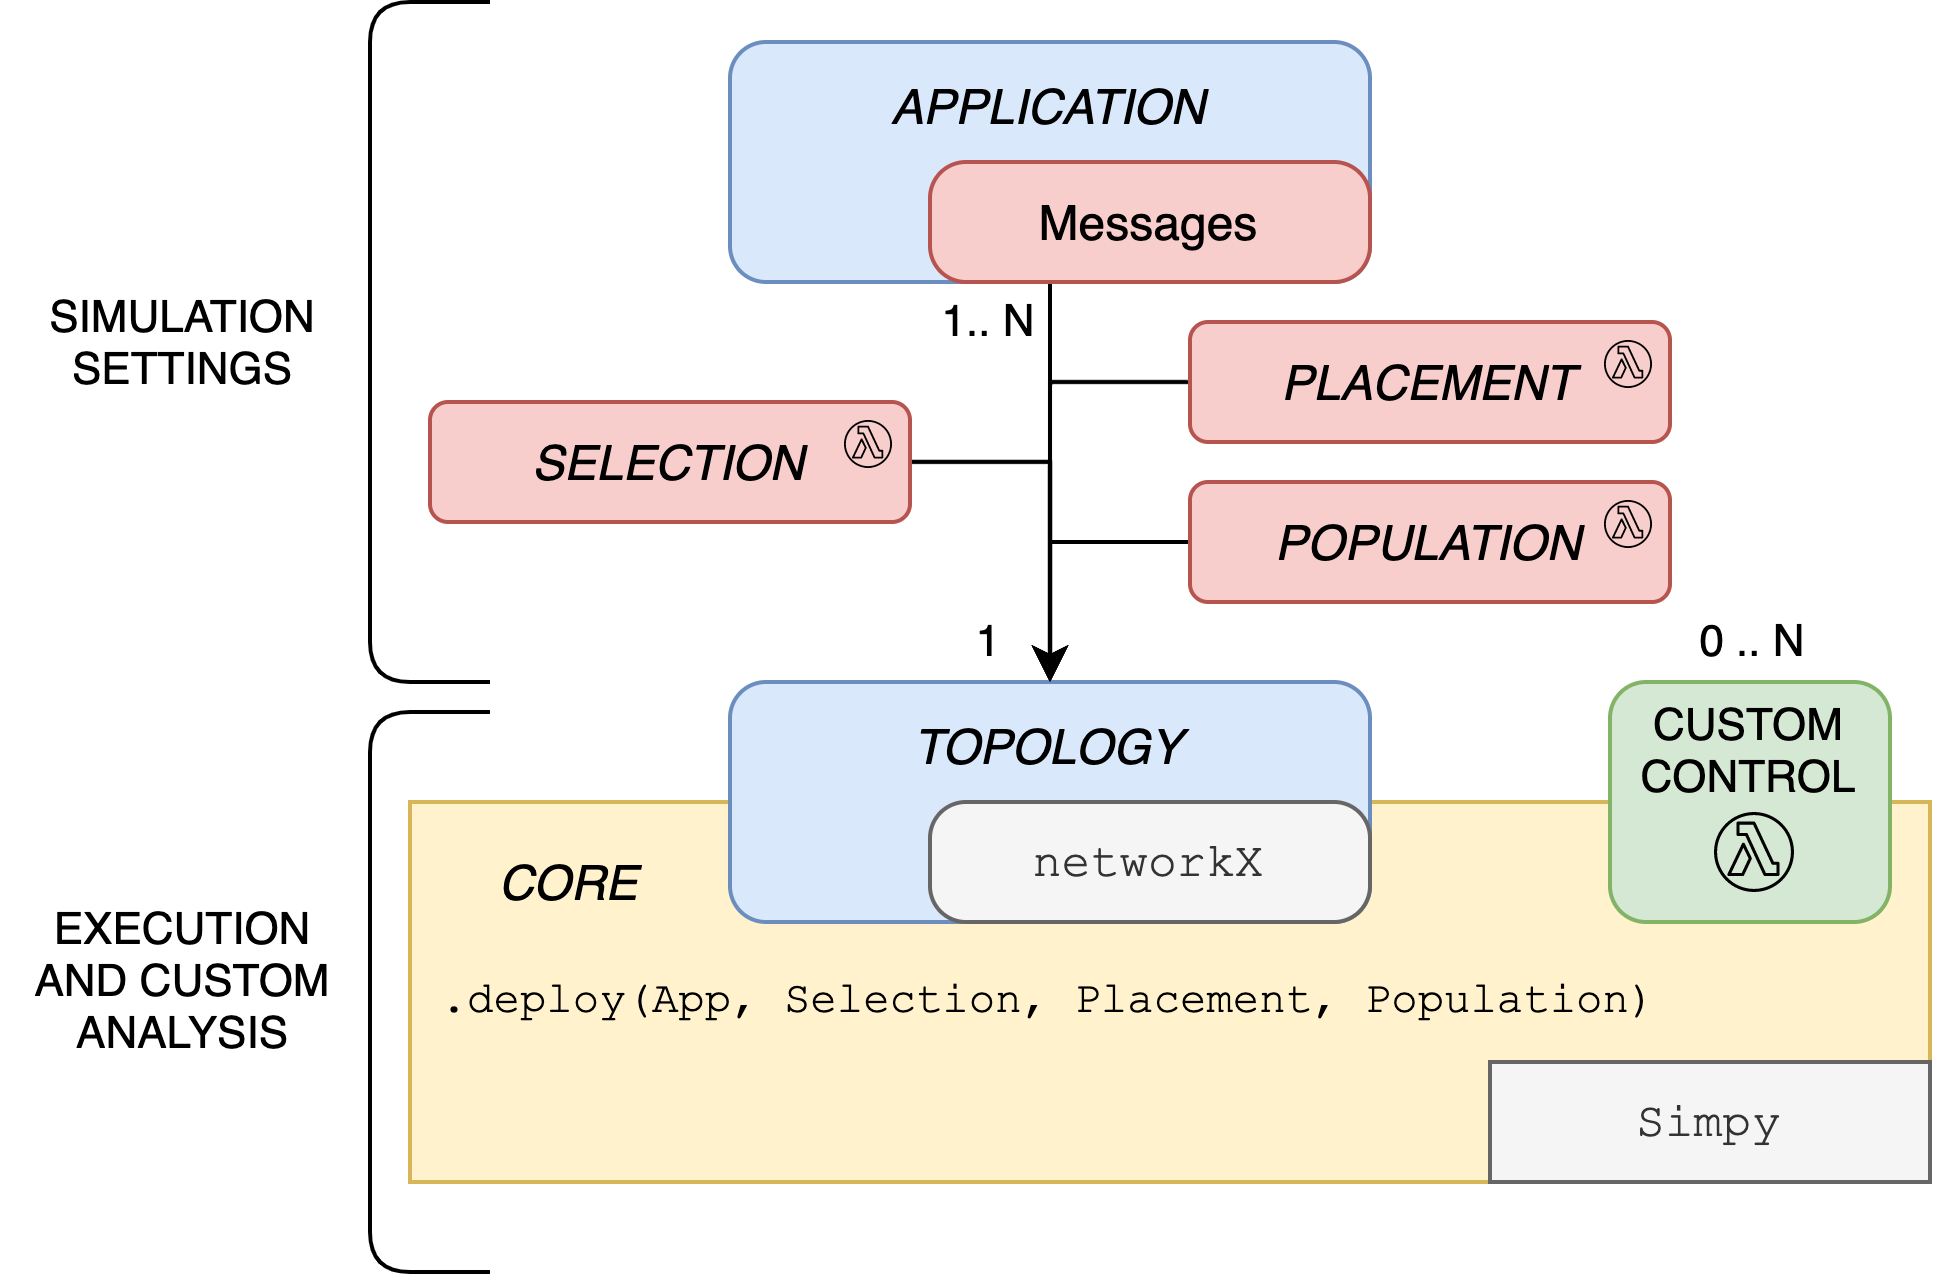
\includegraphics[width=12cm]{images/YAFS_classes}
  \centering
  \caption[Architettura di YAFS]{Architettura di YAFS}
  \label{fig:YAFS_classes}
\end{figure}

\subsection{Topologia e modellazione delle entità}

Le entità della topologia sono modellate come un insieme di \textit{nodi} (ovvero i dispositivi della rete, come dispositivi IoT, nodi fog, server e cloudlet) interconnessi da \textit{archi} (i collegamenti di rete). L'implementazione della topologia, tramite un \textit{grafo}, permette l'applicabilità della \textit{Complex Network Theory} grazie all'integrazione di \textit{NetworkX}  \cite{NetworkX}, una nota libreria, scritta in Python, che fornisce diversi algoritmi per eseguire misure e analisi sui grafi, come degree, centrality, clustering, assortativity, communities e così via. NetworkX accetta inoltre la definizione dei grafi tramite JSON, linguaggio ampiamente utilizzato per la creazione dello scenario con YAFS e permette l'esportazione dei grafi in formato GEXF, utile ad esempio per l'analisi dei grafi tramite il software \textit{Gephi} \footnote{Disponibile su: \url{https://gephi.org/}}.

Gli attributi obbligatori per la definizione di un nodo sono un identificativo univoco (\textit{ID}), il numero di istruzioni eseguite dal nodo in un'unità di tempo (\textit{IPT}) e la capacità della memoria (\textit{RAM}). L'utente è libero di aggiungere attributi personalizzati, utili allo scenario specifico che si vuole studiare (come è stato fatto nel corrente lavoro di Tesi. Maggiori informazioni sono al capitolo \ref{chapter:implementazione}). Un esempio di definizione dei nodi è mostrato nel Listing \ref{lst:node-definition}. 
\begin{lstlisting}[language=json, caption={Definizione di due nodi Fog utilizzando la rappresentazione JSON \cite{YAFSSimulator}}, captionpos=b, label={lst:node-definition}]
{
	"id": 120, "RAM": 1, "IPT": 530,
	"POWERmin": 574,
	"POWERmax": 646,
	"coordinate": 
	{
		"lat": 39.30, "long": 3.34
	}
},
{
	"id": 12, "RAM": 10, "IPT": 100
}
\end{lstlisting}

La definizione dei collegamenti è molto simile. Questi hanno i seguenti attributi obbligatori: la larghezza di banda (\textit{BW}), la velocità di propagazione (\textit{PR}), l'ID del nodo sorgente (\textit{s}) e l'ID del nodo di destinazione (\textit{d}). I valori \textit{BW} e \textit{BR} sono utili al calcolo della latenza secondo la formula:
$$\frac{Message.size.bytes}{BW} + PR$$

\subsection{Modellazione delle Applicazioni}
In YAFS le applicazioni (ovvero dei raggruppamenti di servizi), sono strutturate come dei \textit{Distributed Data Flow} (DDF) \cite{DDF_IOT_App}. In particolare un'applicazione è definita da un insieme di moduli che si scambiano dei messaggi. Infatti, un DDF è rappresentato da un \textit{grafo diretto aciclico}, dove i nodi sono i moduli che eseguono delle azioni sui messaggi in ingresso, provenienti da un certo percorso sugli archi del grafo. Questa rappresentazione è utile al fine di garantire il partizionamento delle applicazioni e la scalabilità, ad esempio tramite l'implementazione di micro-servizi \cite{microservices}. 

\begin{figure}[!ht]
  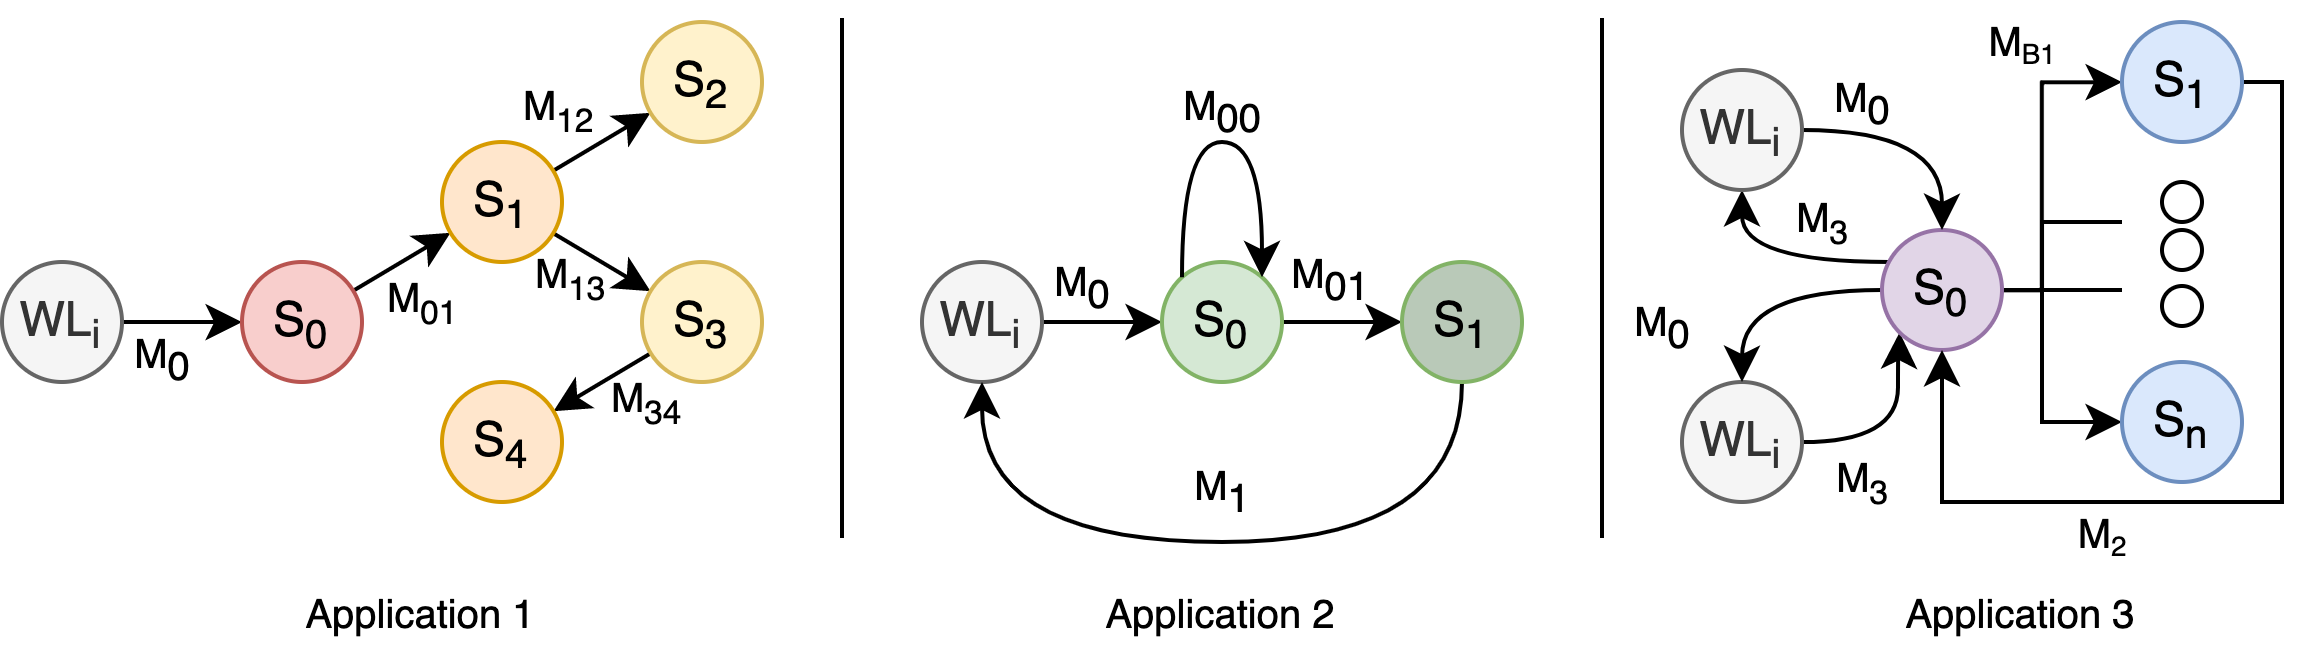
\includegraphics[width=14cm]{images/applications_ddf}
  \centering
  \caption{Tre tipologie di applicazioni realizzabili, con la loro rappresentazione tramite grafo.}
  \label{fig:applications_ddf}
\end{figure}

La definizione delle applicazioni è composta da quattro parti: \textit{moduli} (o \textit{servizi}), \textit{messaggi}, \textit{trasmissioni} e dati generali. I \textit{moduli} possono avere diversi attributi, anche a seconda dello specifico scenario, ma quelli obbligatori sono solo un identificativo univoco (\textit{ID}) e il nome (\textit{name}). I \textit{messaggi}, ovvero i dati scambiati, hanno principalmente due attributi obbligatori: il numero di istruzioni (\textit{instructions}) e la grandezza in byte (\textit{bytes}). Le \textit{trasmissioni} definiscono le modalità in cui i servizi scambiano le informazioni e tramite le quali si inviano dati. Gli attributi obbligatori in questo caso sono: il modulo di afferenza (\textit{module}) e il messaggio in ingresso. Tramite la definizione delle trasmissioni è possibile, con un particolare attributo detto \textit{fractional}, definire la probabilità di propagare un determinato messaggio \textit{message\_out} sulla ricezione di un particolare messaggio \textit{message\_in}. 

In Figura \ref{fig:applications_ddf} sono mostrate tre tipologie di applicazioni che sono realizzabili. La prima, \texttt{Application 1}, è strutturata gerarchicamente, con la ricezione dei messaggi $M_{ij}$ che scatena l'invio di altri messaggi. Nella seconda applicazione, \texttt{Application 2}, è possibile osservare un'interazione di un servizio con se stesso ed infine nell'ultima applicazione, \texttt{Application 3}, è mostrato il \textit{broadcasting} di un messaggio $M_{B1}$ che raggiunge tutti i moduli dell'applicazione. In tutte e tre le applicazioni $WL_i$ indica il nodo che genera il carico di lavoro (ad esempio un dispositivo IoT).

\subsection{Politiche dinamiche}
Le classi \textit{Selection}, \textit{Placement} e \textit{Population} sono utili per la generazione dinamica degli eventi dello scenario. In particolare la prima definisce quali nodi devono eseguire un particolare servizio, di conseguenza indirizza il \textit{workload}. La classe \textit{Placement} sceglie i servizi che devono essere allocati nei vari nodi, mentre la class \textit{Population} posiziona i generatori del workload nei nodi della rete. Queste tre classi possiedono principalmente due interfacce: una contenente l'\textit{initialization function} (che prepara l'allocazione dei moduli e del workload nei nodi della rete) e una contenente una funzione che viene invocata secondo una specifica distribuzione temporale.

\begin{lstlisting}[language=python, caption={Definizione di due Population policies: una statica (\textit{popA}) ed una dinamica (\textit{popB}) \cite{YAFSSimulator}}, captionpos=b, label={lst:population-policy}]
delayActivation = deterministicDistributionStartPoint(300, 300, name='Deterministic')
periodActivation = deterministicDistribution(name='Deterministic', time=100)

popA = Statical(name='StaticalPop')
popA.set_sink_control({'id': a_id_fog_device, 'number': 2, 'module': appA.get_sink_modules()})
popA.set_src_control({'number': 1, 'message': appA.get_message('M.Action'), 'distribution': periodicActivation})

top20Devices = [''array_ids_fog_devices'']
popB = Evolution(top20Devices, name='DynamicPop', activation_dist = delayActivation)
popB.set_sink_control({'model': 'actuator-device', 'number': 2, 'module': appB.get_sink_control()})
popB.set_src_control({'number': 1, 'message': appB.get_message('M.action'), 'distribution': periodicActivation})

\end{lstlisting}

Nel Listing \ref{lst:population-policy} è mostrato un esempio di definizione di politiche di \textit{Population}: una statica ed una dinamica. Nelle righe 1 e 2 vengono definite due distribuzioni temporali: la prima che inizia a 3000 unità temporali e da quel punto in poi invoca un'attivazione ogni 300 unità temporali, la seconda invece che invoca un'attivazione ogni 10 unità temporali. Alla riga 4 viene generata un'istanza di una classe Population predefinita. Le applicazioni YAFS hanno due tipi di moduli: \textit{workload sources} e \textit{workload sinks} (rispettivamente "sensori" ed "attuatori"). Le righe 5 e 6, tramite JSON, definiscono l'allocazione dei moduli sink e dei moduli source con una specifica distribuzione e il tipo di messaggio che questi devono trattare.

Nel caso della seconda politica di \textit{Population}, viene utilizzato un modello più complesso (righe 8-11): alla riga 9 viene istanziato un oggetto Evolution (Listing \ref{lst:population-evolution}). Questo segue la distribuzione di riga 1, dunque, il processo DES creato, inizia a produrre messaggi dopo un certo intervallo di tempo secondo una specifica scadenza. Ad ogni attivazione il processo creato genera workload con le caratteristiche definite alla riga 11.

\begin{lstlisting}[language=python, caption={Struttura di una classe Population \cite{YAFSSimulator}}, captionpos=b, label={lst:population-evolution}]

class Evolution(population):
	def __init__(self, listIDEntities, **kwargs):
		# initialization of internal variables
		super(Evolutionm self).__init__(**kwargs)
	
	def initial_allocation(self, sim, app_name):
		# dealing assignments
		sim.deploy_sink(app_name, node=fog_device, module=module)
	
	def run(self, sim):
		# dealing assignements: msg, distribution and app_name
		id = ... # listIDEntities.next
		idsrc = sim.deploy_source(app_name, id_node=id, msg=..., distribution=...)

\end{lstlisting}

Nel Listing \ref{lst:population-evolution} è mostrata una versione semplificata della classe Evolution. In questo tipo di classi è sempre presente una funzione obbligatoria chiamata \texttt{initial\_allocation} e, facoltativamente, una funzione chiamata \texttt{run} che viene chiamata secondo l'eventuale distribuzione temporale specificata.

\section{Descrizione dello scenario simulato}

L'architettura di riferimento per la definizione dello scenario simulato è esposta in Figura \ref{fig:architettura_scenario}.

\begin{figure}[!ht]
  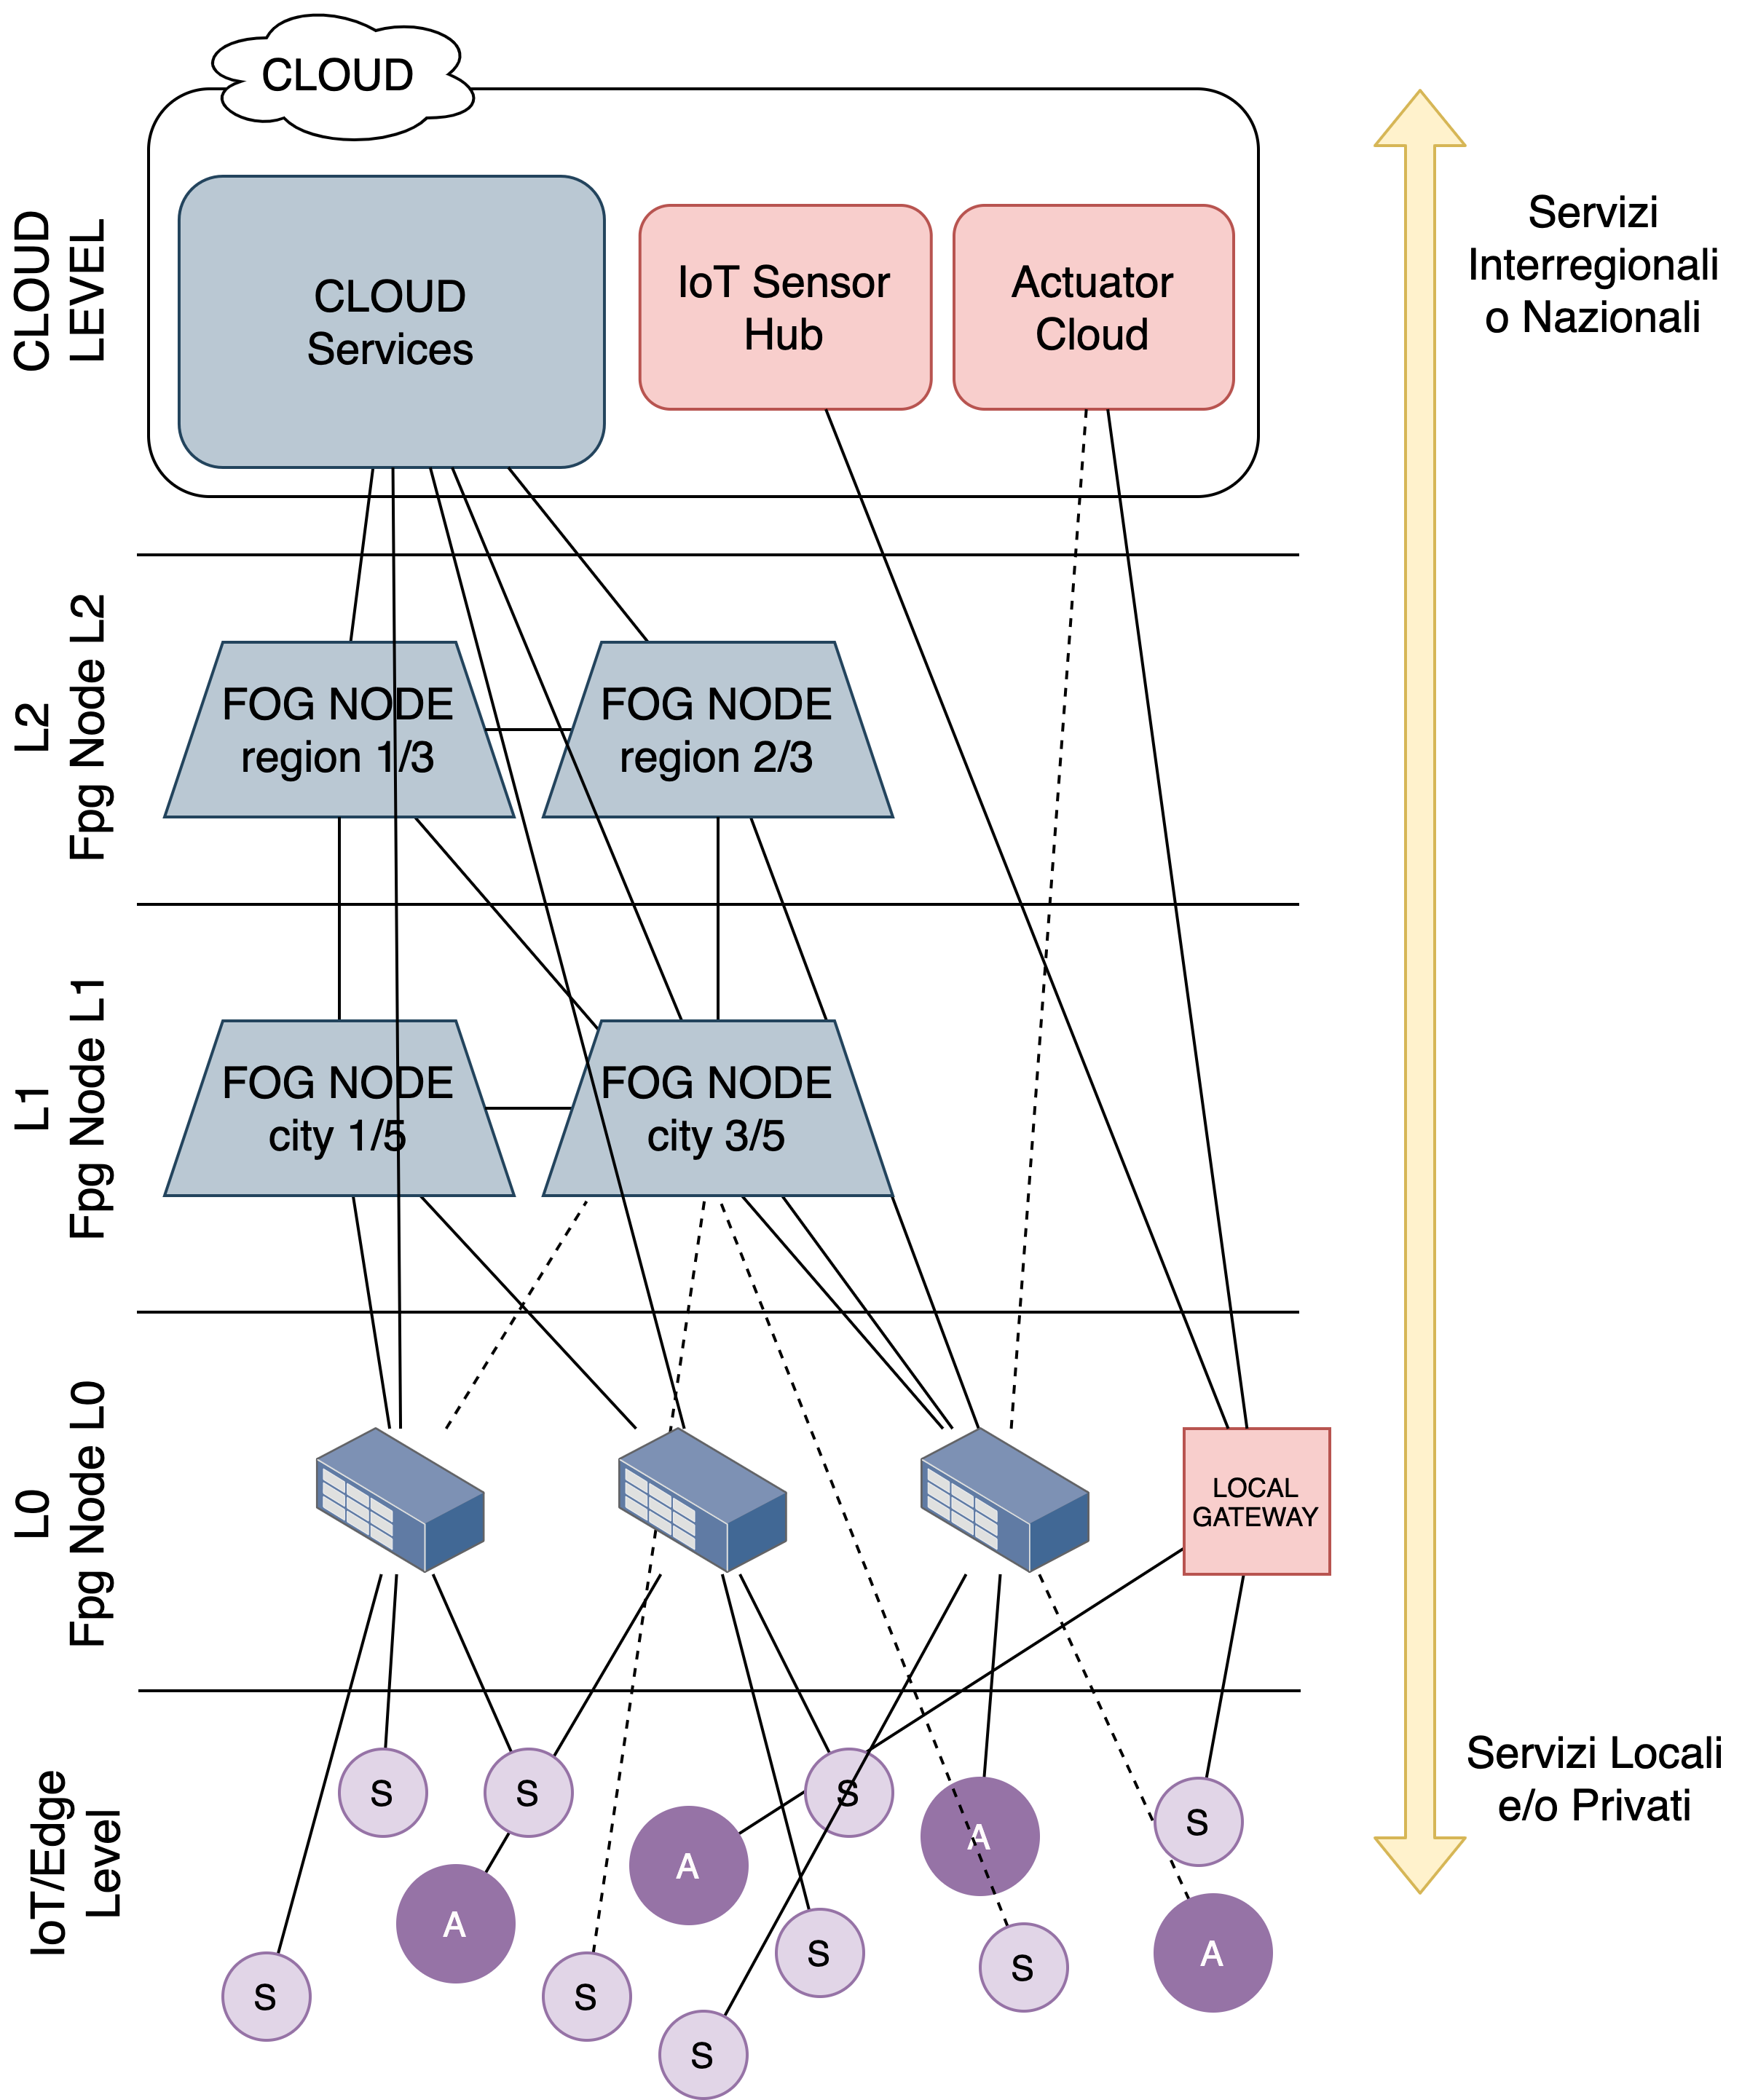
\includegraphics[width=14cm]{images/architettura_scenario}
  \centering
  \caption{Architettura dello scenario simulato}
  \label{fig:architettura_scenario}
\end{figure}

Tra i vari aspetti considerati durante la definizione della topologia di rete si è voluto enfatizzare il concetto del Fog Computing come "architettura verticale". Dall'esempio in Figura \ref{fig:architettura_scenario} è infatti possibile evincere una struttura della rete gerarchica ed a livelli. Ogni livello è caratterizzato da diverse capacità di elaborazione, in base ai servizi offerti alla rete: un nodo a livelli più bassi offre pochi servizi, ma generalmente produce molti dati (ad esempio i dispositivi IoT), mentre un nodo a livelli più alti non genera dati \textit{propri}, ma piuttosto offre una rielaborazione dei dati ricevuti dai livelli più bassi offrendo molti servizi alla rete.

Un fattore di particolare rilevanza è inoltre la \textit{raggiungibilità}. Ricordando infatti la necessità di rendere i servizi della rete disponibili anche nelle zone più remote della stessa, ovvero vicino all'\textit{edge} per ridurre al minimo la latenza, i nodi appartenenti a livelli più bassi sono più radicati nel territorio ed ognuno di essi è raggiungibile da aree via via più limitate e circoscritte. 

\subsection{Architettura a livelli}























         
         \chapter{Sviluppo ed Utilizzo}
\label{chapter:implementazione}

\section[Sistema Realizzato per Simulazioni ed Analisi]{Sistema Realizzato per Simulazioni ed\\ Analisi}
\label{section:sistema_analisi}

Al fine di valutare le prestazioni degli scenari di Fog Computing, descritti al capitolo \ref{chapter:architettura}, è stato implementato un sistema di simulazione che ne permette in una prima fase la definizione in ogni suo aspetto (topologia, applicazioni, servizi, richieste, ecc...) e, successivamente, l'analisi dei principali aspetti utili alla comprensione dello scenario, come il successo del \textit{service placement} e delle richieste di servizi da parte dei vari nodi della rete.

La definizione e l'esecuzione della simulazione seguono il diagramma di flusso mostrato in Figura \ref{fig:sim_flow_diagram}. Come accennato è possibile eseguire due principali tipologie di analisi:
\begin{enumerate}
	\item \textbf{Analisi del service placement}. È possibile analizzare l'andamento del service placement al variare di specifici parametri di definizione dello scenario, specificando il numero di iterazioni e quali di questi devono variare ad ogni esecuzione.
	\item \textbf{Analisi della simulazione}. Una volta definito e simulato uno specifico scenario, è possibile ottenere un'analisi sul soddisfacimento delle richieste da parte dei nodi dei vari servizi offerti dalla rete, con e senza \textit{failure control} dei nodi/servizi.
\end{enumerate}


\begin{figure}[!ht]
  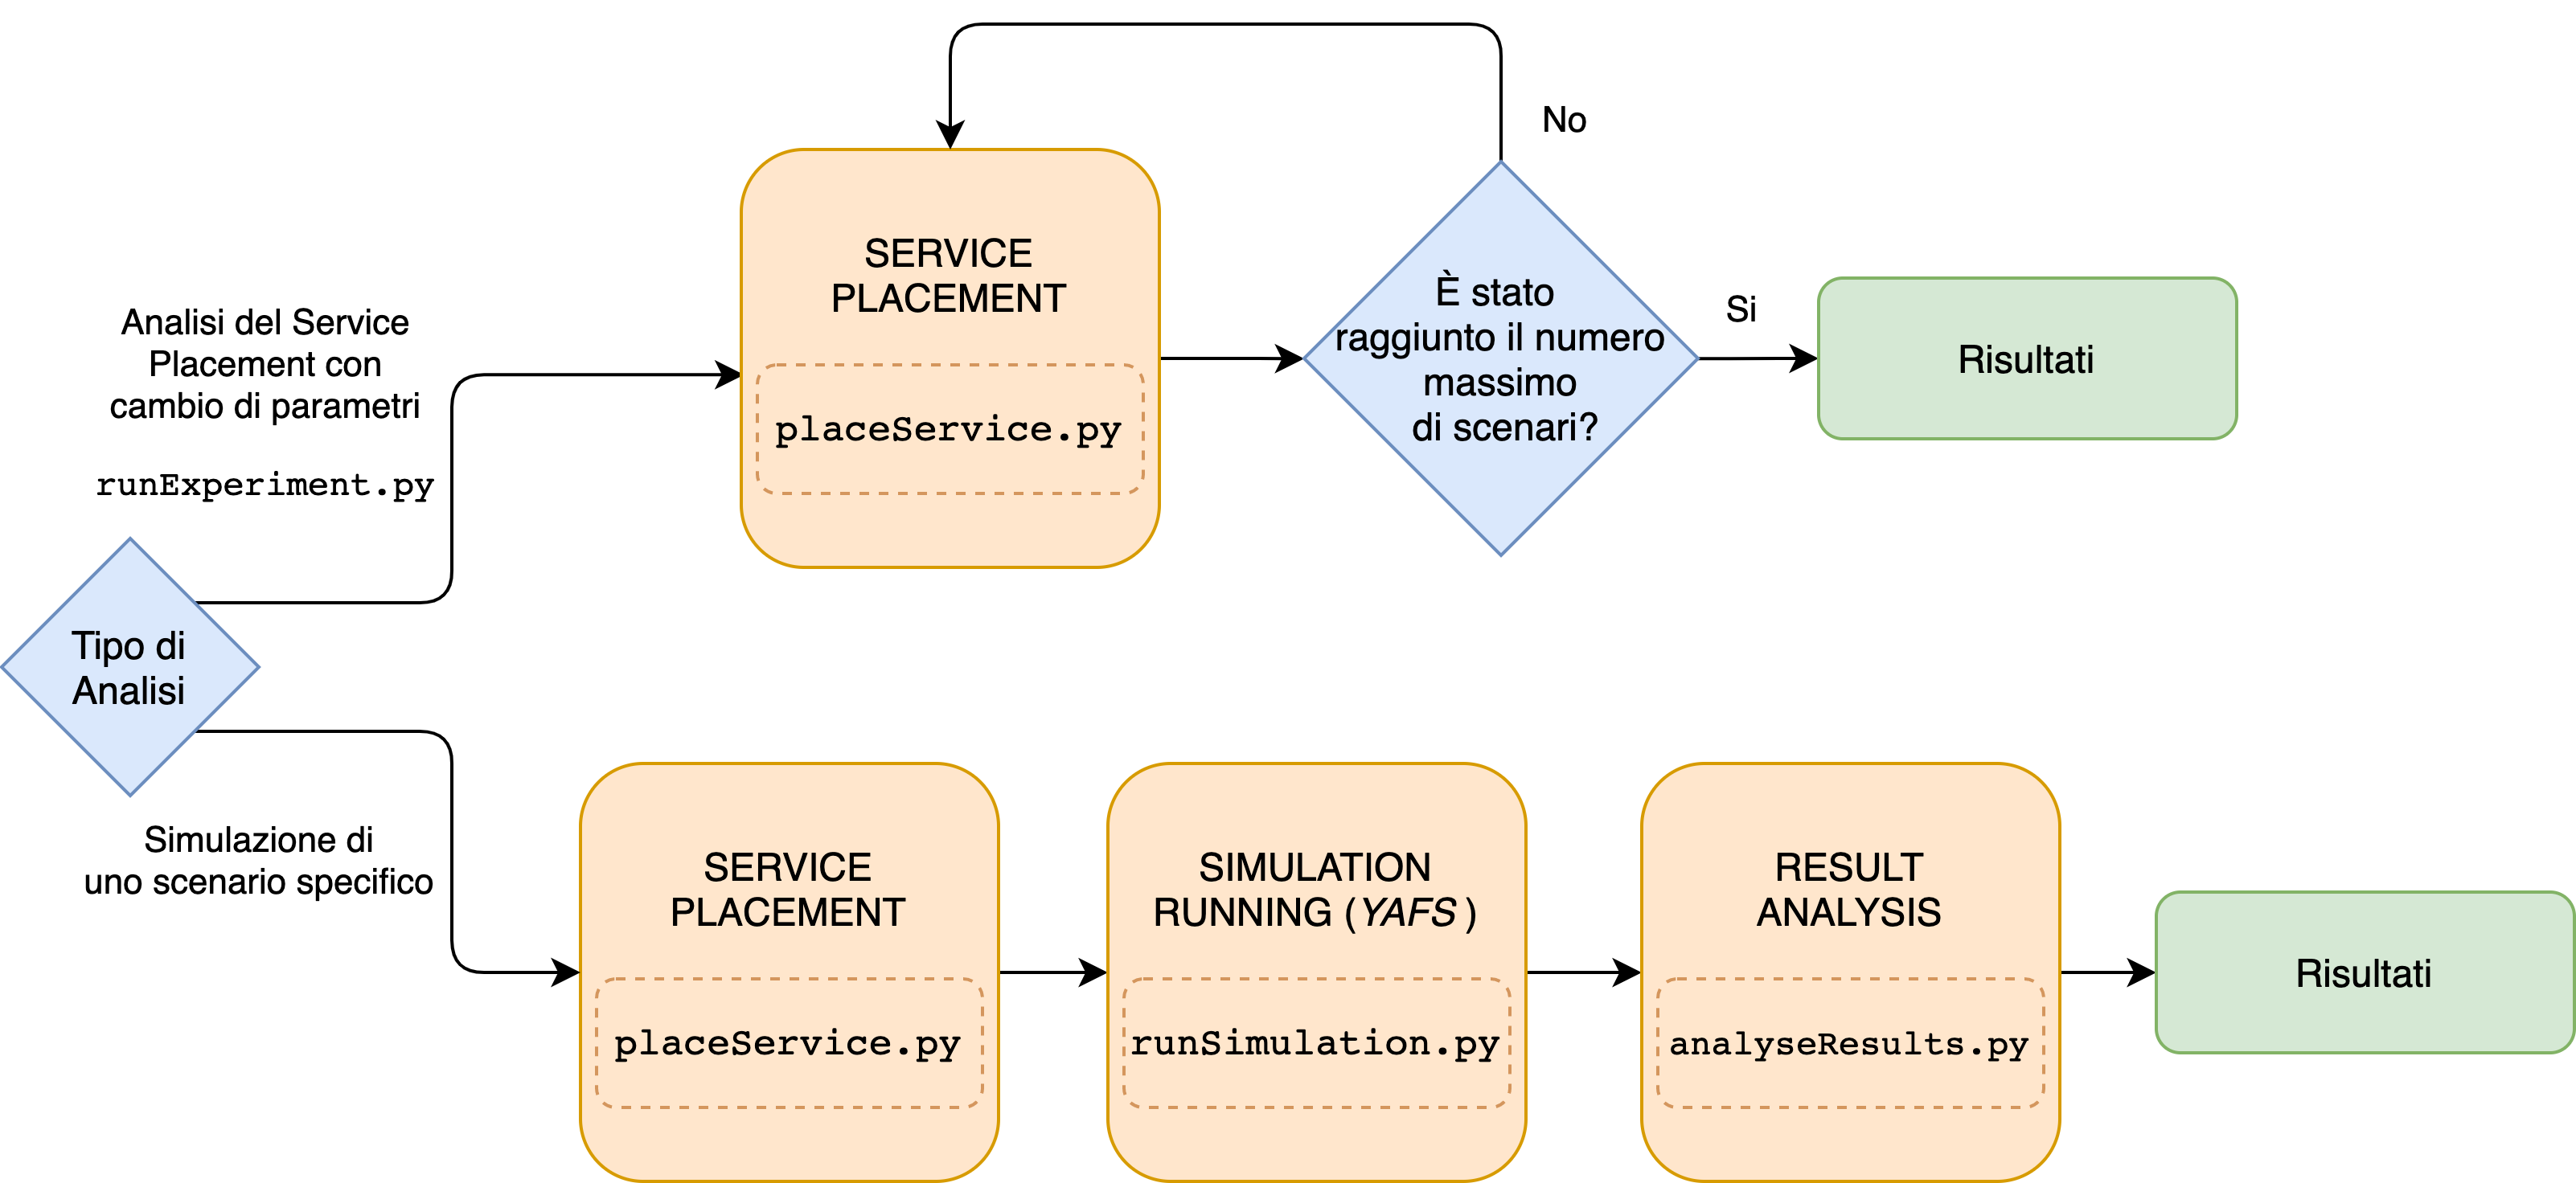
\includegraphics[width=14cm]{images/sim_flow_diagram}
  \centering
  \caption{Diagramma di flusso del sistema di simulazione.}
  \label{fig:sim_flow_diagram}
\end{figure}

\section{Implementazione delle Fasi di Simulazione}

In questo paragrafo verranno approfonditi i singoli aspetti che compongono il processo esposto al Paragrafo \ref{section:sistema_analisi}, nonché il loro utilizzo per la definizione e l'esecuzione delle simulazioni.

\subsection{Service Placement}

Per ottenere il massimo beneficio dall'implementazione di un'architettura Fog, è necessario un efficace algoritmo di \textit{service placement}. In generale questi algoritmi sono improntati a massimizzare il \textit{Quality of Service}\footnote{Con \textit{Quality of Service} si intende l'insieme dei valori che indicano la qualità del servizio offerto dalla rete, in termini di throughput, gestione degli errori, gestione dei ritardi e utilizzo della banda.} (QoS) o il bilanciamento del carico, oppure a minimizzare il consumo di energia, la latenza o il costo della comunicazione.

         \chapter{Risultati}

In questo capitolo verranno presentati i principali risultati ottenuti dalle simulazioni eseguite. Ne sono state effettuate diverse, con varie configurazioni. Verranno valutati l'algoritmo di placement al variare di specifici parametri ed, eventualmente, il soddisfacimento delle richieste con e senza failure control.

\section{Simulazioni con Variazione di Singoli Parametri}

\subsection{Simulazione con Variazione della Privacy}

In questo scenario l'algoritmo di placement è stato eseguito undici volte. Ad ogni esecuzione viene incrementato il valore di privacy di 10 unità, partendo da 0 fino a 100. Si ricorda che il valore di privacy indica il livello massimo, nell'architettura di riferimento, in cui un servizio può essere allocato. Il parametro che varia è in particolare \texttt{PRIVACY\_ASSIGNMENT}. Questo parametro indica la percentuale di servizi a cui il valore di privacy viene assegnato.

Come si può vedere dal grafico in Figura \ref{fig:privacy_placement_success}, l'algoritmo di placement ha un successo accettabile fino ad un valore di privacy pari a 60, con un successo del posizionamento della applicazioni pari al $60\%$. Da questo valore in poi il successo cala drasticamente.

\begin{figure}[!ht]
  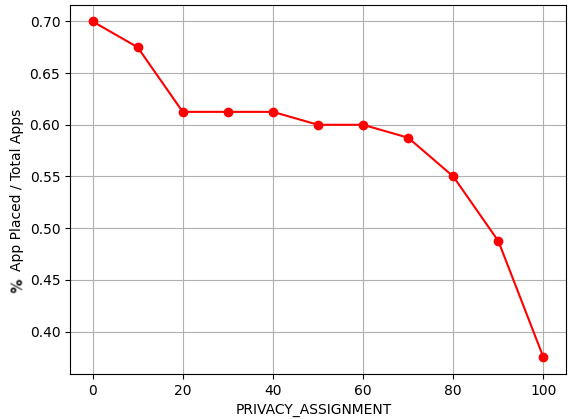
\includegraphics[width=10cm]{images/privacy_placement_success}
  \centering
  \caption{Successo dell'algoritmo di placement al variare del parametro \texttt{PRIVACY\_ASSIGNMENT}.}
  \label{fig:privacy_placement_success}
\end{figure}

Ciò che maggiormente si evince dal grafico in Figura \ref{fig:privacy_placement_per_level} è che il livello Cloud viene utilizzato solo per l'1.5\%. Si ricorda che il compito del Cloud è quello di fungere da nodo utile per i servizi che non hanno trovato un nodo Fog disponibile in fase di placement. Il valore di privacy non può quindi crescere troppo.

\begin{figure}[!ht]
  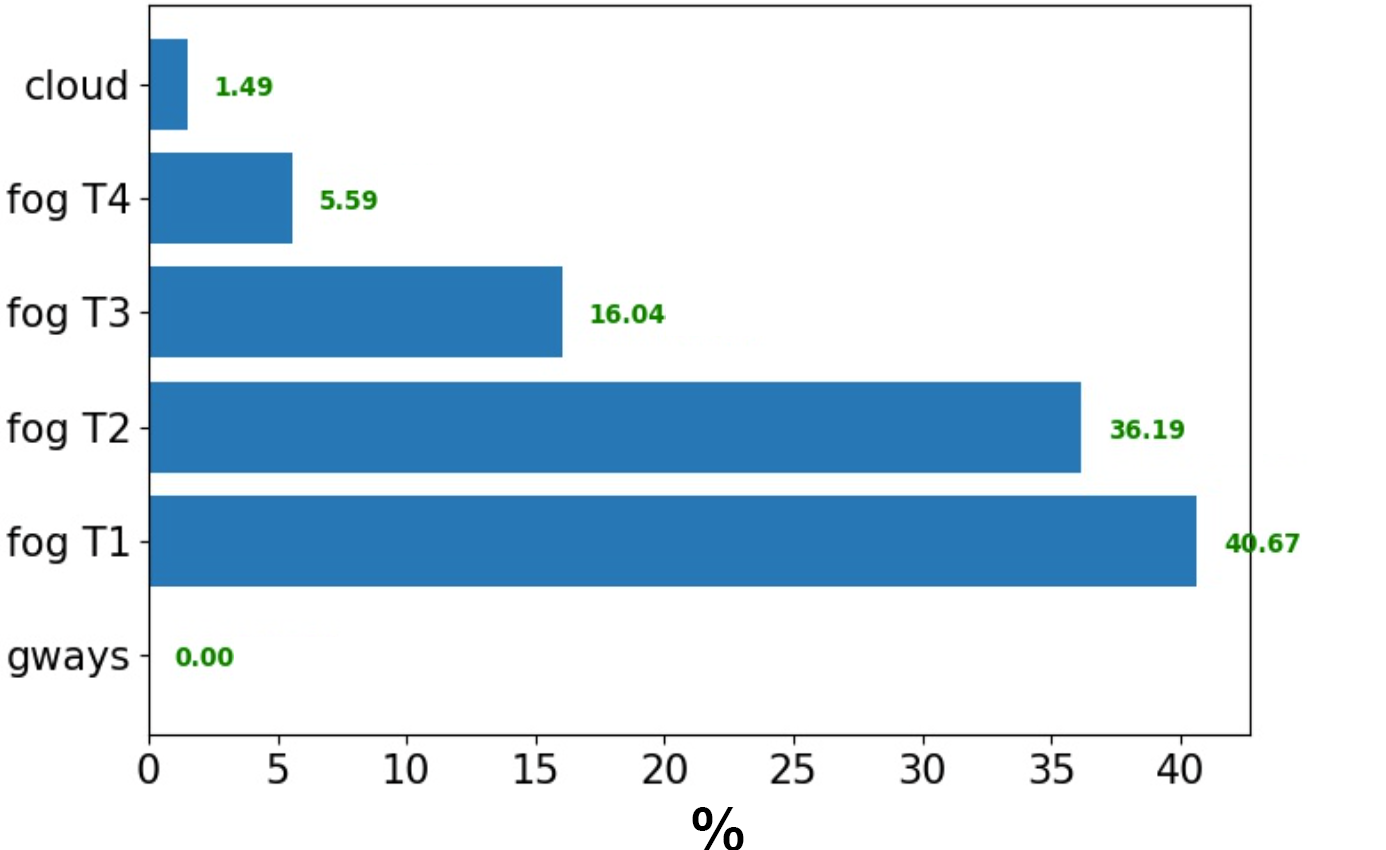
\includegraphics[width=10cm]{images/privacy_placement_per_level}
  \centering
  \caption{Percentuale di servizi allocati in ogni livello.}
  \label{fig:privacy_placement_per_level}
\end{figure}

È stata inoltre valutato, con questo valore di privacy, il soddisfacimento delle richieste con e senza failure control. Questo risultato è mostrato nel grafico in Figura \ref{fig:privacy70_simulation_result}.

\begin{figure}[!ht]
  \includegraphics[width=14cm]{images/privacy70_simulation_result}
  \centering
  \caption{Numero di richieste soddisfatte durante la simulazione, con e senza failure control.}
  \label{fig:privacy70_simulation_result}
\end{figure}

\subsection{Simulazione con Variazione delle Risorse Richieste dai Servizi}

In questo scenario l'algoritmo di placement è stato eseguito dieci volte. Ad ogni esecuzione viene incrementato il valore corrispondente alle risorse richieste dai servizi. Il parametro in questione è \texttt{FUNC\_SERVICE\_RESOURCES}. Il successo dell'algoritmo di placement al variare di tale parametro è mostrato nel grafico in Figura \ref{fig:resources_placement_success}. Il risultato principale che si evince dal grafico è la velocità con il quale decresce la percentuale di applicazioni correttamente allocate. Infatti aumentando, anche di poco, il numero di risorse richieste poche applicazioni vengono allocate.

\begin{figure}[!ht]
  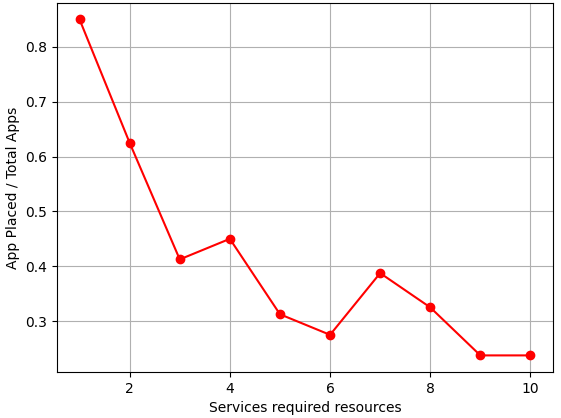
\includegraphics[width=10cm]{images/resources_placement_success}
  \centering
  \caption{Successo dell'algoritmo di placement al variare del parametro \texttt{FUNC\_SERVICE\_RESOURCES}.}
  \label{fig:resources_placement_success}
\end{figure}

È stata eseguita una simulazione con \texttt{FUNC\_SERVICE\_RESOURCES} pari a \texttt{random.randint(7, 10)}. Le risorse allocate per livello sono mostrate nel grafico in Figura \ref{fig:resources_placement_per_level}. In questo caso come si evince dal grafico in Figura \ref{fig:resources_placement_success}, sono state allocate correttamente circa il 40\% delle applicazioni.

\begin{figure}[!ht]
  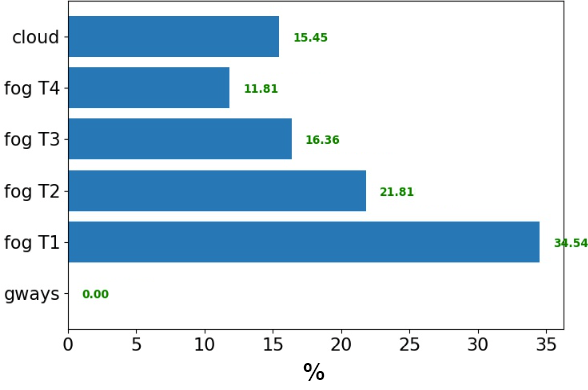
\includegraphics[width=10cm]{images/resources_placement_per_level}
  \centering
  \caption{Percentuale di servizi allocati in ogni livello}
  \label{fig:resources_placement_per_level}
\end{figure}

\subsection{Simulazione con Variazione del Fattore di Riduzione dei Nodi nei Livelli Superiori}

In questo scenario l'algoritmo di placement è stato eseguito 21 volte, facendo variare il parametro \texttt{REDUCTION\_FACTOR\_2}, incrementandolo di 0.1 ad ogni iterazione. Questo parametro regola la riduzione del numero di nodi Fog da un livello a quello successivo. Quando \texttt{REDUCTION\_FACTOR\_2} è pari a 1 il numero di nodi Fog non varia, viceversa quando questo valore è pari a 3 il numero di nodi Fog ad un determinato livello $n$ sarà pari ad $1/3$ del numero di nodi del livello $n-1$.

I risultati dell'esecuzione consecutiva dell'algoritmo di placement è mostrato nel grafico in Figura \ref{fig:YAFS_classes}

\begin{figure}[!ht]
  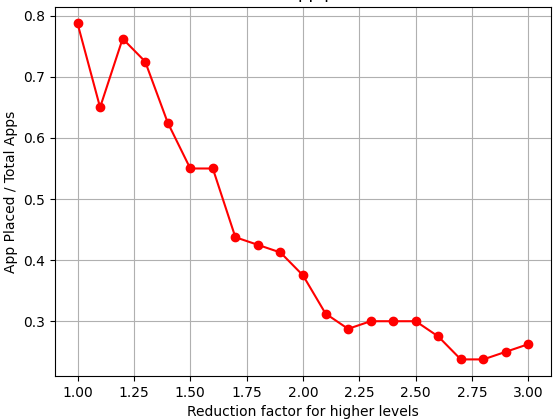
\includegraphics[width=10cm]{images/nodes_number_placement_success}
  \centering
  \caption{Successo dell'algoritmo di placement al variare del parametro \texttt{REDUCTION\_FACTOR\_2}.}
  \label{fig:nodes_number_placement_success}
\end{figure}

Ciò che si evince dal grafico è che, salvo alcune oscillazioni, la tendenza è fortemente decrescente. Infatti oltre al valore 1.5 il successo dell'algoritmo di placement cala drasticamente. 

Per evidenziare quanto detto vengono riportati in Figura \ref{fig:reduction_factor_placement_comparison} i grafici raffiguranti la percentuale di servizi correttamente allocati per ogni livello. A destra viene mostrato il grafico ottenuto impostando il valore di \texttt{REDUCTION\_FACTOR\_2} pari a 1, a sinistra pari a 3. 

Ciò che si evince è che l'algoritmo di placement, grazie alla sua natura greedy, ha allocato in entrambi i casi la percentuale maggiore di servizi nel primo livello. Nel primo caso però molti servizi sono stati allocati nei livelli superiori, con una percentuale che differisce di poche unità, mentre nei livelli superiori, dato il numero molto più basso di nodi disponibili, dove cala drasticamente il successo di placement, cala conseguentemente anche il numero di servizi per livello.

\begin{figure}[!ht]
  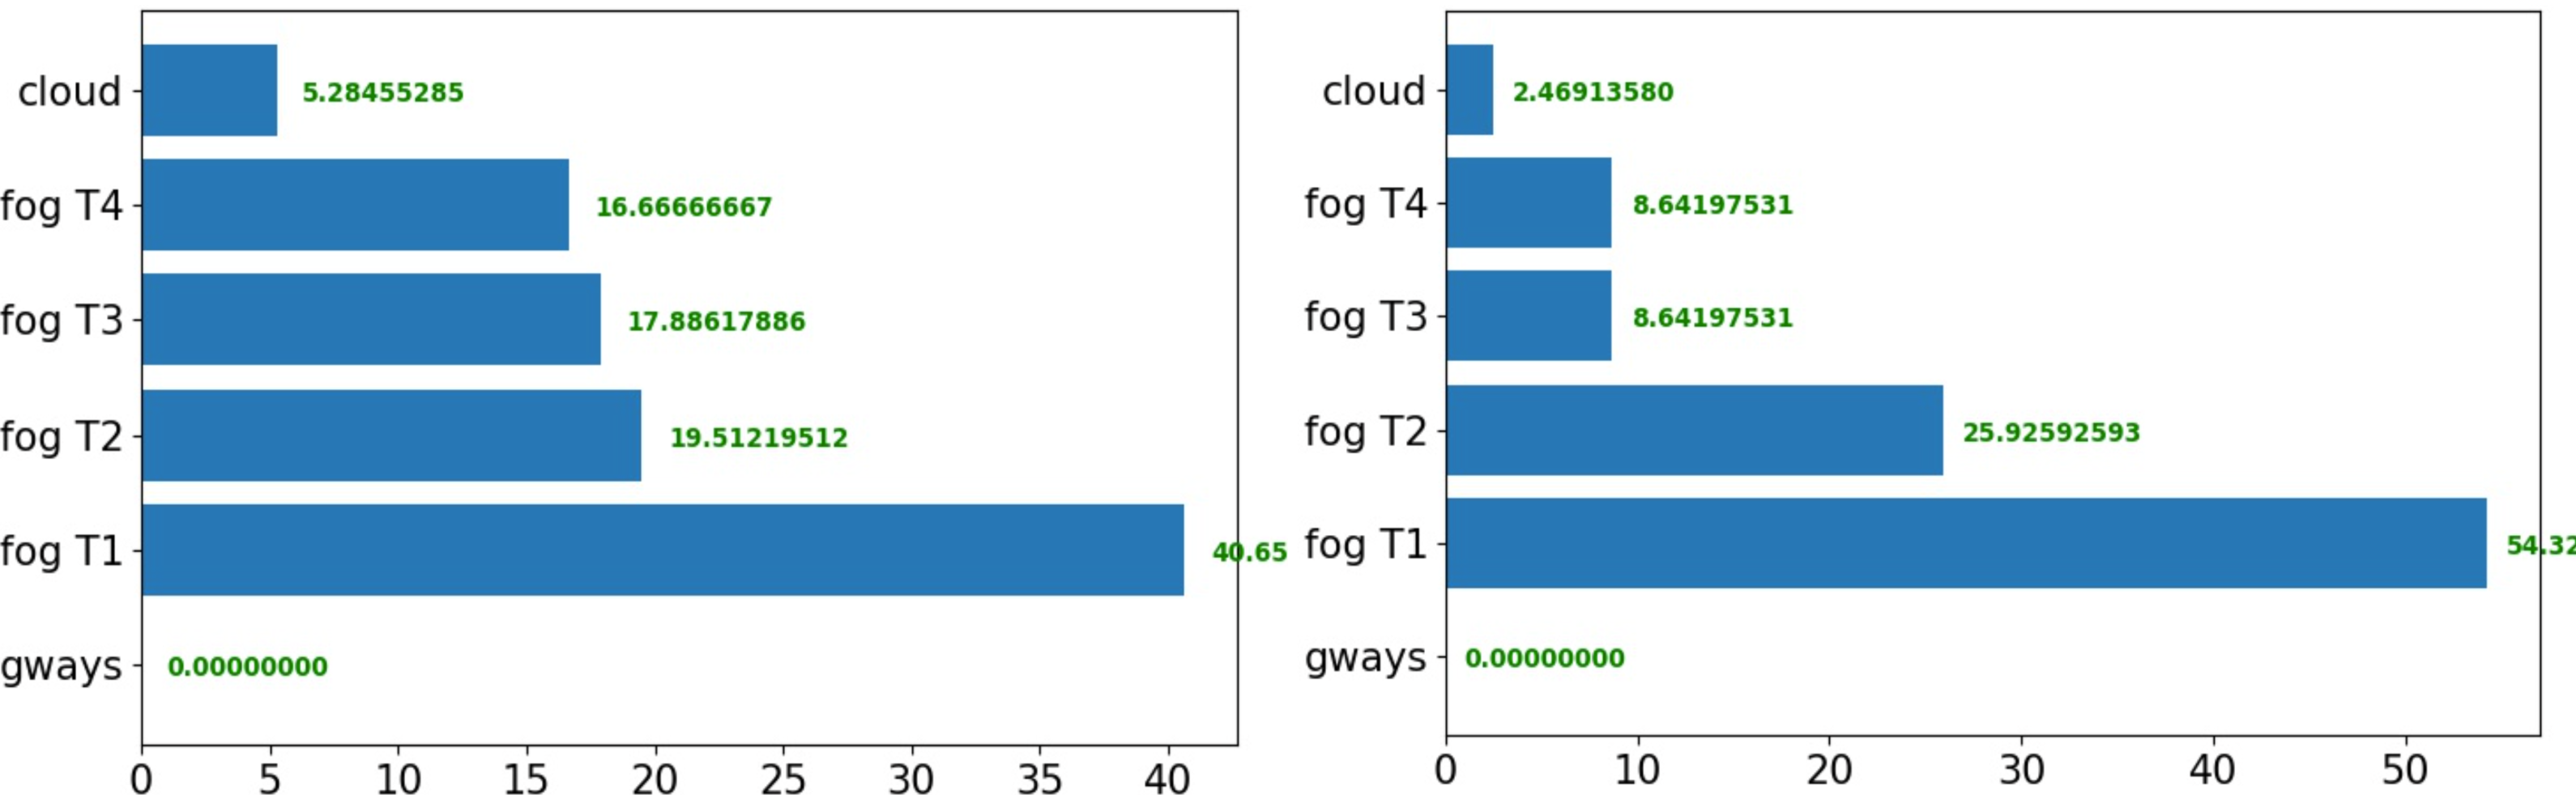
\includegraphics[width=14cm]{images/reduction_factor_placement_comparison}
  \centering
  \caption{Percentuale di servizi correttamente allocati in ogni livello. A sinistra con \texttt{REDUCTION\_FACTOR\_2} pari a 1, a destra con \texttt{REDUCTION\_FACTOR\_2} pari a 3.}
  \label{fig:reduction_factor_placement_comparison}
\end{figure}

\subsection{Simulazione con Variazione del Numero di Connessioni dai Livelli Inferiori ai Livelli Superiori}

In questo scenario è stato eseguito 20 volte l'algoritmo di placement facendo variare il numero di connessioni di ogni nodo dai livelli inferiori ai livelli superiori. In particolare sono stati fatti variare i variare i parametri \texttt{MIN\_CONN\_TO\_UPPER\_LEVELS} e \texttt{MAX\_CONN\_TO\_UPPER\_LEVELS} da 10 e 20, rispettivamente, a 200 e 210.

Il successo del placement al variare di tali parametri è mostrato nel grafico in Figura \ref{fig:minmax_conn_to_upper}

\begin{figure}[!ht]
  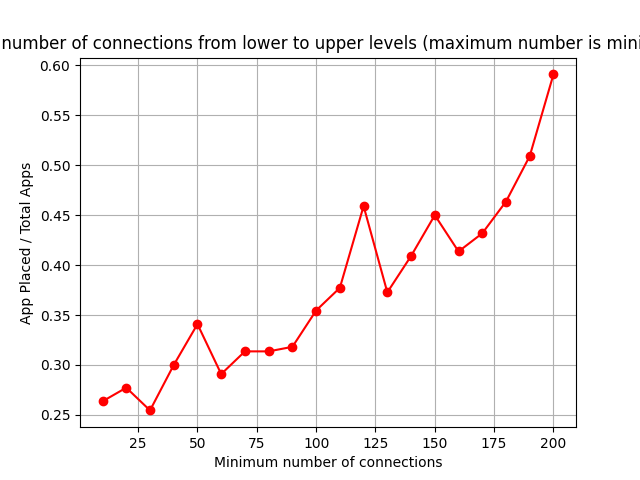
\includegraphics[width=10cm]{images/minmax_conn_to_upper}
  \centering
  \caption{Successo dell'algoritmo di placement al variare del parametro \texttt{MIN\_CONN\_TO\_UPPER\_LEVELS}.}
  \label{fig:minmax_conn_to_upper}
\end{figure}

Dal grafico si evince che all'aumentare del valore relativo al numero minimo di coonnesioni verso i livelli più alti aumenta il successo dell'algoritmo di placement. Il fattore di maggiore rilevanza è rappresentato dal fatto che all'aumentare delle connessioni verso i livelli alti vengono garantite un numero sempre maggiore di strade per poter allocare servizi ai nodi più alti. Per sottolineare quanto detto, sono stati eseguite due simulazioni, una con \texttt{MIN\_CONN\_TO\_UPPER\_LEVELS = 10} e \texttt{MAX\_CONN\_TO\_UPPER\_LEVELS = 20}, l'altra con \texttt{MIN\_CONN\_TO\_UPPER\_LEVELS = 200} e \texttt{MAX\_CONN\_TO\_UPPER\_LEVELS = 210}. Per ognuna delle due sono stati prodotti i grafici, mostrati in Figura \ref{fig:min_conn_to_upper_levels_comparison}, relativi alla percentuale di servizi che vengono allocati nei vari livelli.

\begin{figure}[!ht]
  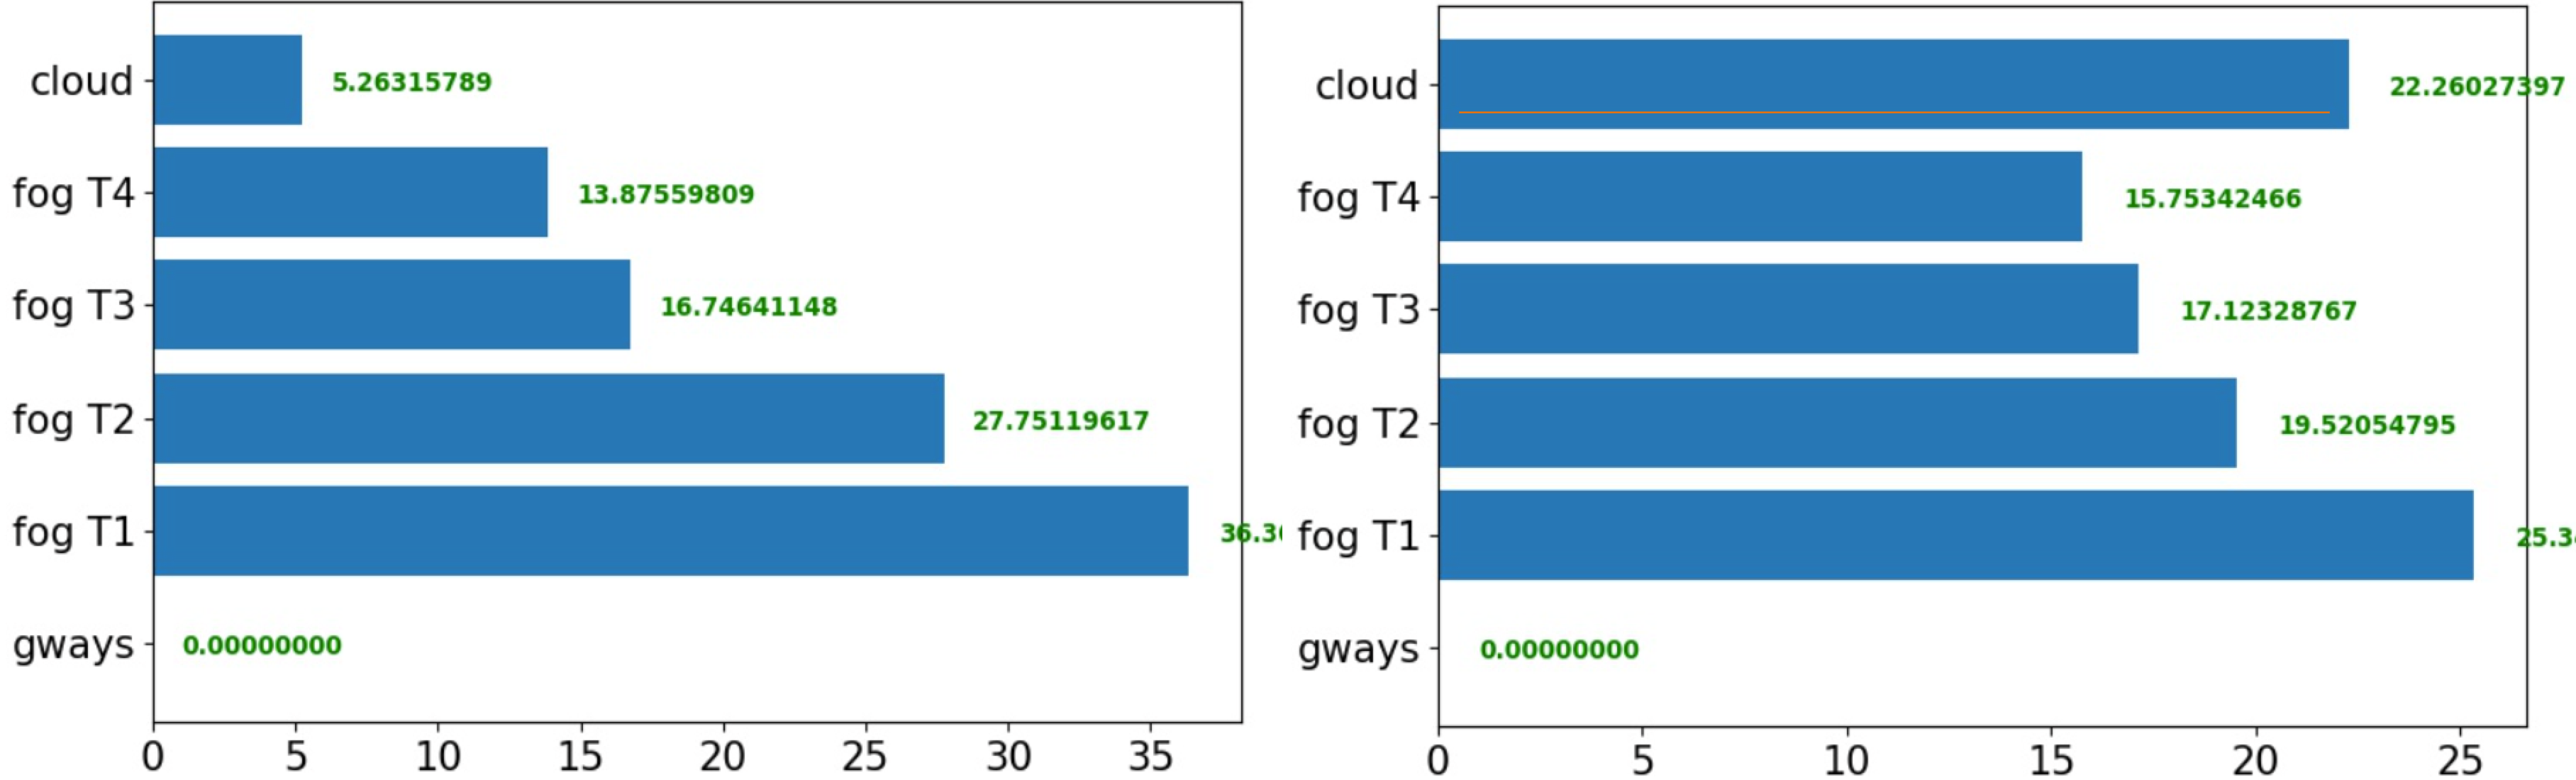
\includegraphics[width=14cm]{images/min_conn_to_upper_levels_comparison}
  \centering
  \caption{Percentuale di servizi correttamente allocati in ogni livello. A sinistra con \texttt{MIN\_CONN\_TO\_UPPER\_LEVELS = 20}, a destra con \texttt{MIN\_CONN\_TO\_UPPER\_LEVELS = 200} pari a 3.}
  \label{fig:min_conn_to_upper_levels_comparison}
\end{figure}

Per valutare il \textit{fault tollerance} della rete sono state eseguite due simulazioni e le rispettive analisi, valutando il soddisfacimento delle richieste prima nello scenario con \texttt{MIN\_CONN\_TO\_UPPER\_LEVELS = 10} e \texttt{MAX\_CONN\_TO\_UPPER\_LEVELS = 20} (Figura \ref{fig:min_conn_20_sim_2}) e poi nello scenario con \texttt{MIN\_CONN\_TO\_UPPER\_LEVELS = 200} e \texttt{MAX\_CONN\_TO\_UPPER\_LEVELS = 210} (Figura \ref{fig:min_conn_200_sim_1}).

\begin{figure}[!ht]
  \includegraphics[width=14cm]{images/min_conn_10_sim_2}
  \centering
  \caption{Numero di richieste soddisfatte durante la simulazione, con e senza failure control.}
  \label{fig:min_conn_20_sim_2}
\end{figure}

\begin{figure}[!ht]
  \includegraphics[width=14cm]{images/min_conn_200_sim_1}
  \centering
  \caption{Numero di richieste soddisfatte durante la simulazione, con e senza failure control.}
  \label{fig:min_conn_200_sim_1}
\end{figure}

 \clearpage

          \chapter*{Conclusioni}
% \chapter* -> the introduction isn't the Chapter 1, it's not a numbered chapter
\addcontentsline{toc}{chapter}{Conclusioni} % this line enable the introduction to be listed in the Table Of Contents even if it's not a numbered chapter (see above)
\markboth{}{}

L'obiettivo di questo lavoro di Tesi è stato la realizzazione di un software di simulazione e valutazione di specifici scenari di implementazione del Fog Computing. Lo strumento sviluppato si è dimostrato piuttosto flessibile, permettendo la valutazione dei diversi aspetti architetturali e di configurazione dei sistemi Fog. Il Fog Computing è caratterizzato da un approccio distribuito, derivante dal bisogno di superare i limiti dell'approccio centralizzato del Cloud Computing. Infatti i nodi Fog possono essere posizionati ovunque nella rete tra gli end-node e il Cloud. Questa flessibilità apre molti interrogativi che possono essere fugati tramite software di simulazione come quello realizzato. 

Sono stati ottenuti diversi risultati rilevanti, come l'andamento del successo dell'algoritmo di placement dei servizi al variare della distribuzione della privacy, delle risorse richieste dai servizi, dell'interconnessione tra i nodi a livello Fog, del numero di questi nodi, e del numero di servizi per ogni applicazione. Questo ha permesso di chiarire quali sono i parametri che più influenzano il successo dell'algoritmo, anche valutando le prestazioni durante la simulazione di un sistema così configurato.

La stesura di questa Tesi nasce da un periodo di Internato di Laboratorio nel quale è stato fatto un lavoro di ricerca sugli aspetti trattati nel Capitolo 1 e che sono serviti per la definizione delle simulazioni, della topologia di rete e per l'analisi dei risultati. Il software realizzato, però, si presta a diverse tipologie di analisi: si può pensare ad un'implementazione di un'architettura differente, di un diverso algoritmo di placement, o a diversi tipi di applicazioni che possono essere allocate nella rete. 

L'IoT ha accelerato la cosiddetta ``trasformazione digitale" e fornisce benefici sia ai singoli utenti che alle aziende di diversi settori, come energia, trasporti, istruzione, sanità pubblica e così via. Proprio grazie all'IoT, il numero di dispositivi connessi è in forte crescita e con questo anche la quantità di dati che vengono prodotti.

Il Fog Computing, unitamente alle sue principali estensioni esposte nel Capitolo 1, si offre come una delle soluzioni più promettenti per la gestione dei Big Data che vengono prodotti dai dispositivi IoT.











\clearpage

\appendix
\renewcommand{\chaptermark}[1]{\markboth{{\appendixname}\ \thechapter.\hspace{1em}#1}{}}

\chapter{Appendice}



\clearpage

\addcontentsline{toc}{chapter}{Bibliografia}
\bibliographystyle{unsrt}
\nocite{*}
\bibliography{riferimenti}
% 
\clearpage

\end{document}


